\documentclass[ba]{imsart}
\RequirePackage{amsthm,amsmath,amsfonts,amssymb}
\RequirePackage[authoryear]{natbib}
\RequirePackage[hypertexnames=false,colorlinks,citecolor=blue,urlcolor=blue]{hyperref}
\RequirePackage{graphicx,booktabs,longtable,multirow,bm,mathtools,microtype,placeins,array}
\RequirePackage{cleveref}
\pubyear{2026}
\startlocaldefs
\theoremstyle{plain}
\newtheorem{lemma}{Lemma}
\newtheorem{proposition}{Proposition}
\newtheorem{corollary}{Corollary}
\theoremstyle{definition}
\newtheorem{assumption}{Assumption}
\newtheorem{remark}{Remark}
\newcommand{\E}{\mathbb{E}}
\newcommand{\Ek}{\mathbb{E}_k}
\newcommand{\Ezeta}{\mathbb{E}_{\zeta}}
\newcommand{\F}{\mathcal{F}}
\newcommand{\norm}[1]{\left\|#1\right\|}
\newcommand{\inner}[2]{\langle #1,\, #2 \rangle}
\newcommand{\calO}{\mathcal{O}}
\makeatletter
\newcommand{\legacytheoremlabel}[2]{\begingroup\def\@currentlabel{#1}\label{#2}\endgroup}
\makeatother
\endlocaldefs
\begin{document}
\begin{frontmatter}
\title{Second-Order Control Variates for Stochastic Gradient Langevin Dynamics}
\runtitle{Second-Order Control Variates for SGLD}
\begin{aug}
\author[A]{\fnms{Michelle}~\snm{Le}},
\author[B]{\fnms{Frank}~\snm{Fan}},
\author[A]{\fnms{Jay}~\snm{Chooi}}
\and
\author[A]{\fnms{Alexander}~\snm{Young}}
\address[A]{Harvard University}
\address[B]{Massachusetts Institute of Technology}
\runauthor{M. Le, F. Fan, J. Chooi and A. Young}
\end{aug}
\begin{abstract}
Second-order control variates reduce the minibatch noise in stochastic-gradient Langevin sampling by subtracting an anchor-based linear approximation to each observation's gradient. We study when this reduction improves posterior accuracy and measured time-to-accuracy under fixed full-Hessian preconditioning. The theoretical analysis develops anchor-distance-dependent gradient-noise and Wasserstein bounds. Our experiments distinguish gradient precision, posterior approximation and setup-inclusive computational cost. On synthetic logistic targets, second-order control variates improve variance estimation without uniformly improving transport discrepancy or time-to-accuracy. On the original Bank Marketing target, rare, high-leverage Taylor remainders trigger numerical failures; controlled single-step interventions identify their mechanism. After a declared feature transformation and symmetric bounded tuning, independently validated configurations yield substantial CPU time-to-accuracy gains. In a nested synthetic dataset-size study, raw gradient-noise scaling agrees qualitatively with the predicted orders, but setup-inclusive speedup declines overall as sample size increases. A cost decomposition explains the decline through shared setup costs and first-order retuning. Gaussian checks verify numerical gradient and trajectory equivalence with full-gradient Langevin sampling. These findings identify conditional benefits and practical limitations rather than universal superiority.
\end{abstract}
\begin{keyword}
\kwd{stochastic-gradient Langevin dynamics}
\kwd{control variates}
\kwd{posterior sampling}
\kwd{preconditioning}
\kwd{computational efficiency}
\end{keyword}
\end{frontmatter}
\section{Introduction}
Stochastic gradient Langevin dynamics (SGLD) replaces the full posterior gradient by a minibatch estimate to make Bayesian computation feasible on large datasets \citep{welling2011}. The resulting subsampling noise is distinct from the injected Langevin noise. First-order control variates anchor the stochastic gradient at a reference point, reducing its variability near that anchor \citep{baker2017}. A second-order control variate additionally cancels the local linear variation of each observation's gradient. The resulting estimator and its theoretical analysis are developed in Sections~\ref{sec:method} and~\ref{sec:theory}.

Our experimental question is when this additional variance reduction improves the accuracy--cost tradeoff of posterior sampling. We focus on a fixed inverse Hessian of the negative log posterior at the anchor, including prior curvature and declared numerical regularization. This separates the gradient-estimator comparison from online adaptive-metric dynamics. Full-gradient unadjusted Langevin sampling (ULA) supplies a diagnostic control for the contribution of stochastic gradients, without being treated as a zero-error posterior sampler.

The empirical evidence has three complementary parts. First, frozen German Credit and logistic-regression comparisons establish accuracy improvements as well as unmet efficiency criteria. Second, an original Bank Marketing failure motivates implementation checks and controlled observation-level interventions. These identify a high-leverage Taylor-remainder mechanism; a transformed-target study then tests the optimized accuracy--cost frontier with independent validation. Third, a nested synthetic study examines dataset-size scaling of both gradient noise and tuned wall-clock cost. A focused Gaussian experiment verifies algebraic exactness and the geometry correction separately from practical speedup.

Together these experiments support conditional computational benefits. They also explain why noise reduction can fail to deliver an advantage: rare large updates, discretization error, grid resolution, competing parameter choices and shared setup costs all matter. We retain unfavorable results and distinguish original primary comparisons from historically motivated extensions and post-result sensitivity analyses.

\section{Related Works}\label{sec:related}
SGLD was introduced by \citet{welling2011}. The control-variate construction of \citet{baker2017} is the first-order baseline extended here. Inaccurate-gradient Langevin bounds provide context for the theoretical analysis \citep{dalalyan2017}, and Hessian--vector products provide a general implementation route for curvature corrections \citep{pearlmutter1994}. The experiments use cached likelihood curvature where practical, while measuring the full posterior Hessian required for the sampling metric.

Adaptive preconditioning is a distinct approach. \citet{li2016psgld} combine an evolving gradient-based diagonal metric with SGLD. Our primary comparisons instead share a fixed full-Hessian metric across CV1, CV2 and full-gradient ULA, holding posterior geometry constant to isolate stochastic-gradient variance reduction. CV2's cached anchor likelihood Hessian can be reused for this metric after adding prior curvature and the declared regularization; all methods are charged for their required metric preparation. Combining control variates with an adaptive metric introduces additional choices about accumulator inputs, initialization and adaptive drift corrections. Those choices are outside the primary comparison. Earlier adaptive controls are retained for completeness, without a general conclusion about Li et al.'s method. Full-data Hamiltonian Monte Carlo (HMC) supplies approximate reference draws \citep{neal2012hmc}; their quality is assessed using rank-based convergence and effective-sample-size diagnostics \citep{vehtari2021rank}.

\section{Method}
\label{sec:method}

\subsection{Setup and Baker's SLGD-CV}
We work with a posterior $\pi(\theta)\propto e^{-U(\theta)}$ on $\mathbb R^d$ whose negative log-density decomposes as
\begin{equation}
  U(\theta) \;=\; U_0(\theta) \;+\; \sum_{i=1}^N U_i(\theta),
  \label{eq:decomp}
\end{equation}
with $U_0$ the prior's contribution and each $U_i$ the contribution of data point $i$. SGLD takes steps
\begin{equation}
  \theta_{k+1} \;=\; \theta_k \;-\; h\,\nabla\tilde U(\theta_k) \;+\; \sqrt{2h}\,\zeta_{k+1}, \qquad \zeta_{k+1}\sim\mathcal N(0,I_d),
  \label{eq:sgld}
\end{equation}
where $h>0$ is the step size, $\zeta_{k+1}$ is an injected standard-Gaussian noise independent of $\theta_k$ and of all past randomness, and $\nabla\tilde U(\theta_k)$ is a stochastic estimate of $\nabla U(\theta_k)$. Throughout, $S_k=(i_1,\dots,i_n)$ denotes the mini-batch at step $k$: an ordered tuple of indices drawn i.i.d.\ uniformly on $\{1,\dots,N\}$ with replacement. For any oracle $\nabla\tilde U$ we write $\xi_k:=\nabla\tilde U(\theta_k)-\nabla U(\theta_k)$ for the \emph{oracle noise}, and for any two probability measures $\mu,\nu$ on $\mathbb R^d$ with finite second moments, $W_2(\mu,\nu)$ denotes the 2-Wasserstein distance.


\textbf{Baker's SGLD-CV.} Fix an \emph{anchor} $\hat\theta\in\mathbb R^d$, typically the output of SGD or L-BFGS run on $U$, so $\hat\theta$ approximates the posterior mode $\theta^\star:=\arg\min_\theta U(\theta)$. Baker's estimator precomputes the full-data anchor gradient $\nabla U_{\text{data}}(\hat\theta):=\sum_{i=1}^N\nabla U_i(\hat\theta)$ and at each step returns
\begin{equation}
  \nabla\tilde U_{\mathrm B}(\theta_k) \;=\; \nabla U_0(\theta_k) \;+\; \nabla U_{\text{data}}(\hat\theta) \;+\; \frac{N}{n}\sum_{j=1}^n\bigl[\nabla U_{i_j}(\theta_k) - \nabla U_{i_j}(\hat\theta)\bigr].
  \label{eq:baker}
\end{equation}
A datum-by-datum conditional expectation confirms $\mathbb E[\nabla\tilde U_{\mathrm B}(\theta_k)\mid\theta_k]=\nabla U(\theta_k)$, so~\eqref{eq:baker} is unbiased. Under per-datum Lipschitz gradients with constants $L_i$, the oracle-noise variance of Baker's estimator scales \emph{quadratically} with distance from the anchor:
\begin{equation}
  \mathbb E\bigl[\|\xi_k^{\mathrm B}\|^2\mid\theta_k\bigr] \;\le\; \frac{M_L^2}{n}\,\|\theta_k-\hat\theta\|^2, \qquad M_L^2:=N^2\bar L^2,\ \bar L^2:=\tfrac{1}{N}\sum_{i=1}^N L_i^2
  \label{eq:baker-var}
\end{equation}
When \(\theta_k\) is far from \(\hat\theta\), which happens on ill-conditioned posteriors whose bulk mass does not concentrate at the anchor, then the right-hand side grows, and the variance reduction degrades.

\subsection{The SGLD-CV2 Estimator}

We replace Baker's zeroth-order anchor $\nabla U_i(\hat\theta)$ with a \emph{first-order Taylor expansion} of each per-datum gradient around $\hat\theta$. Define the second-order control variate for the data terms by
\begin{equation}
  C_k \;=\; \frac{N}{n}\sum_{j=1}^n\!\bigl[\nabla U_{i_j}(\hat\theta) + \nabla^2 U_{i_j}(\hat\theta)(\theta_k-\hat\theta)\bigr],
\end{equation}
whose conditional expectation is
\begin{equation}
  \mathbb E[C_k\mid\theta_k] \;=\; \nabla U_{\text{data}}(\hat\theta) \;+\; \nabla^2 U_{\text{data}}(\hat\theta)(\theta_k-\hat\theta),
\end{equation}
where $\nabla^2 U_{\text{data}}(\hat\theta):=\sum_{i=1}^N\nabla^2 U_i(\hat\theta)$ is the summed full-data Hessian at the anchor. Applying the control-variate formula $(N/n)\sum_j\nabla U_{i_j}(\theta_k)-C_k+\mathbb E[C_k\mid\theta_k]$ to the data terms and adding back the exact prior gradient gives the SGLD-CV2 oracle:
\begin{equation}
  \boxed{\;\nabla\tilde U_{\mathrm{CV2}}(\theta_k) \;=\; \nabla U_0(\theta_k) \;+\; \nabla U_{\text{data}}(\hat\theta) \;+\; \nabla^2 U_{\text{data}}(\hat\theta)(\theta_k-\hat\theta) \;+\; \frac{N}{n}\sum_{j=1}^n r_{i_j}(\theta_k),\;}
  \label{eq:cv2}
\end{equation}
where the \emph{per-datum Taylor remainder} is
\begin{equation}
  r_i(\theta) \;:=\; \nabla U_i(\theta) - \nabla U_i(\hat\theta) - \nabla^2 U_i(\hat\theta)(\theta-\hat\theta).
  \label{eq:remainder}
\end{equation}

The estimator~\eqref{eq:cv2} has three pieces. The prior gradient $\nabla U_0(\theta_k)$ is evaluated exactly at every step and contributes no variance. The deterministic second-order Taylor term $\nabla U_{\text{data}}(\hat\theta)+\nabla^2 U_{\text{data}}(\hat\theta)(\theta_k-\hat\theta)$ is precomputed once (up to one $d\times d$ matrix--vector product per step) and contributes no variance. The stochastic remainder $(N/n)\sum_j r_{i_j}(\theta_k)$ is the sole source of variance.

\textbf{Unbiasedness.} By construction, $\mathbb E[\nabla\tilde U_{\mathrm{CV2}}(\theta_k)\mid\theta_k]=\nabla U(\theta_k)$. Indeed, \[\mathbb E[(N/n)\sum_j\nabla U_{i_j}(\theta_k)\mid\theta_k]=\nabla U_{\text{data}}(\theta_k),\] and the Taylor-term cancellation in~\eqref{eq:cv2} completes the identity.

\textbf{Reduction to Baker.} Setting $\nabla^2 U_i(\hat\theta)=0$ for all $i$ zeros out every Hessian term in~\eqref{eq:cv2} and recovers Baker's~\eqref{eq:baker}. In this sense SGLD-CV is the special case of SGLD-CV2 with the curvature correction dropped.

\subsection{Algorithm}
\label{sec:algorithm}


Given the posterior decomposition~\eqref{eq:decomp} and a fixed step size $h>0$, SGLD-CV2 performs a one-off preprocessing step followed by samplingas per usual.

\noindent\fbox{\parbox{0.98\linewidth}{%
\textbf{SGLD-CV2.}

\textbf{Preprocessing.}
\begin{enumerate}\setlength\itemsep{2pt}\vspace{-4pt}
  \item Run an optimizer (e.g. SGD) to obtain an anchor $\hat\theta$ approximating $\theta^\star$.
  \item Cache per-datum anchor gradients $g_i:=\nabla U_i(\hat\theta)$ for $i=1,\dots,N$ and their sum $\nabla U_{\text{data}}(\hat\theta)=\sum_i g_i$.
  \item Cache the summed full-data Hessian at the anchor, $H_{\text{data}}:=\nabla^2 U_{\text{data}}(\hat\theta)\in\mathbb R^{d\times d}$.
\end{enumerate}

\textbf{Sampling.} Initialize $\theta_0=\hat\theta$. For $k=0,1,2,\dots$:
\begin{enumerate}\setlength\itemsep{2pt}\vspace{-4pt}
  \setcounter{enumi}{3}
  \item Draw mini-batch $S_k=(i_1,\dots,i_n)$. For each $j$, compute $\nabla U_{i_j}(\theta_k)$, look up $g_{i_j}$ from Step 2, and compute the per-datum Hessian-vector product $\nabla^2 U_{i_j}(\hat\theta)(\theta_k-\hat\theta)$ via \citet{pearlmutter1994}.
  \item Form $\nabla\tilde U_{\mathrm{CV2}}(\theta_k)$ by~\eqref{eq:cv2} with $H_{\text{data}}(\theta_k-\hat\theta)$ in place of $\nabla^2 U_{\text{data}}(\hat\theta)(\theta_k-\hat\theta)$.
  \item Update $\theta_{k+1}=\theta_k - h\,\nabla\tilde U_{\mathrm{CV2}}(\theta_k) + \sqrt{2h}\,\zeta_{k+1}$, $\zeta_{k+1}\sim\mathcal N(0,I_d)$.
\end{enumerate}
}}%


\section{Theoretical Analysis}
\label{sec:theory}
\subsection{Wasserstein bound}
Because SGLD targets a continuous distribution, we need a metric that quantifies how close the distribution $\nu_k$ of the $k$-th iterate is to the true posterior $\pi$. The 2-Wasserstein distance $W_2(\nu_k,\pi)$ is a natural choice: it metrizes weak convergence while accounting for the geometry of the parameter space, and its squared form admits a clean coupling argument that translates the oracle-noise variance of our gradient estimator directly into a recursive bound on sampling error. Controlling $W_2$ therefore lets us compare SGLD-CV2 against Baker's SGLD-CV on equal footing and makes the benefit of the quartic variance bound (\Cref{prop:quartic}) precise in terms of the distribution's actual distance to stationarity.
From lectures, our sampling target is:
$$
    \pi(\theta) \propto e^{-U(\theta)}, \quad \theta \in \mathbb{R}^d,
$$
where $U : \mathbb{R}^d \to \mathbb{R}$ is differentiable.
Recall the overdamped Langevin diffusion:
$$
    d\theta_t = -\nabla U(\theta_t)\,dt + \sqrt{2}\,dB_t.
$$
In the integral form:
$$
    \theta_t = \theta_0 - \int_0^t \nabla U(\theta_s)\,ds + \sqrt{2}\,B_t.
$$
From \citet{welling2011}:
$$U(\theta) = U_0(\theta) + \sum_{i=1}^N U_i(\theta)$$
where $U_0(\theta) = -\log p(\theta)$ is the prior term and $U_i(\theta) = -\log p(y_i \mid \theta)$ are the likelihood terms. And so:
\begin{align}
    \nabla U(\theta) &= \nabla U_0(\theta) + \sum_{i=1}^N \nabla U_i(\theta), \\
    \nabla^2 U(\theta) &= \nabla^2 U_0(\theta) + \sum_{i=1}^N \nabla^2 U_i(\theta).
\end{align}
At each iteration, SGLD uses the mini-batch gradient
\begin{equation}
    \nabla \tilde{U}(\theta_k) = \nabla U_0(\theta_k) 
    + \frac{N}{n}\sum_{i \in S_k} \nabla U_i(\theta_k)
\end{equation}
where $S_k \subset \{1,\ldots,N\}$ is a uniformly sampled mini-batch of size 
$|S_k| = n$. This is an unbiased estimator of the full-batch gradient, i.e. $\mathbb{E}_{S_k}\!\left[\nabla \hat{U}(\theta_k)\right] = \nabla U(\theta_k)$.

Our proposed \textbf{second-order control variate} is:
$$C_k = \frac{N}{n}\sum_{i \in S_k} [\nabla U_i(\hat\theta) + \nabla^2 U_i(\hat\theta)(\theta_k - \hat\theta)]$$
with deterministic expectation 
$$\mathbb{E}[C_k] = \left[\nabla U(\hat\theta) - \nabla U_0(\hat\theta)\right] + \left[\nabla^2 U(\hat\theta) - \nabla^2 U_0(\hat\theta)\right](\theta_k - \hat\theta)$$
Applying $\nabla\hat{U}_{\text{CV2}}(\theta_k) = \nabla\tilde{U}(\theta_k) - C_k + \mathbb{E}[C_k]$ as a control-variated unbiased estimator of the full-batch gradient:
\begin{align}
\nabla\hat{U}_{\text{CV2}}(\theta_k) 
    &= \nabla U_0(\theta_k) + \bigl[\nabla U(\hat\theta) 
        + \nabla^2 U(\hat\theta)(\theta_k - \hat\theta)\bigr] - \bigl[\nabla U_0(\hat\theta) 
        + \nabla^2 U_0(\hat\theta)(\theta_k - \hat\theta)\bigr] \notag\\
    &\quad + \frac{N}{n}\sum_{i \in S_k}\bigl(\nabla U_i(\theta_k) 
        - \nabla U_i(\hat\theta) 
        - \nabla^2 U_i(\hat\theta)(\theta_k - \hat\theta)\bigr).
    \label{eq:cv2-theory}
\end{align}
% \jay{I think we have duplicate expositions above on SGLD-CV2 with section 3. Michelle since you put this in first, feel free to trim mine.}
\begin{assumption}\label{ass:convex}[Strongly log-concave target, i.e.\ strongly convex potential]
There exist positive constants $m$ and $M$ such that the following holds for the potential $U$:
\begin{align}
    U(\theta) - U(\theta') - \nabla U(\theta')^\top (\theta - \theta') &\geq \frac{m}{2} \|\theta - \theta'\|^2 \\
    \|\nabla U(\theta) - \nabla U(\theta')\| &\leq M \|\theta - \theta'\|.
\end{align}
for all $\theta, \theta' \in \mathbb{R}^d$.
\end{assumption}
We further need a Lipschitz condition for each of the likelihood terms in order to bound the variance of our control-variate estimator of the gradient.
\begin{assumption}[Lipschitz Gradients]
\label{ass:grad}
    There exist constants $L_0, \ldots, L_N$ such that
\begin{equation}
    \|\nabla U_i(\theta) - \nabla U_i(\theta')\| \leq L_i \|\theta - \theta'\|, 
    \quad \text{for } i = 0, \ldots, N.
\end{equation}
\end{assumption}
\begin{assumption}[Lipschitz Hessians]
\label{ass:hess}
    There exist constants $M_0, \ldots, M_N$ such that
\begin{equation}
|\nabla^2 U_i(\theta) - \nabla^2 U_i(\theta')| \leq M_i |\theta - \theta'|, \quad \text{for } i = 0, \ldots, N.
\end{equation}
\end{assumption}

Using \Cref{ass:hess} we are able to derive a bound on the variance of the gradient estimate of SGLD-CV. This bound is formally stated in Proposition 1.

\begin{proposition}\label{prop:quartic}
\textit{Under Assumption 3. Let $\theta_k$ be the state of SGLD-CV2 at the $k^{th}$ 
iteration, with stepsize $h$ and centering value $\hat\theta$. Assume we estimate 
the gradient using the second-order control variate estimator. Define $\xi_k := \nabla \hat{U}(\theta_k) - \nabla U(\theta_k)$, 
so that $\xi_k$ measures the noise in the gradient estimate $\nabla \hat{U}$ 
and has mean $0$. Then for all $\theta_k, \hat{\theta} \in \mathbb{R}^d$, for all 
$k = 1, \ldots, K$ we have}
\begin{equation}\label{eq:lemma1}
\mathbb{E}\|\xi_k\|^2 \leq \frac{N}{4n} \left( \sum_{i=1}^N M_i^2 \right) \mathbb{E}\|\theta_k - \hat\theta\|^4.
\end{equation}
\end{proposition}

\begin{proof}
Our proof follows similarly to \citet{baker2017}.
Note that:
$$\nabla^2 U(\hat\theta)(\theta_k - \hat\theta) = \sum_{i=1}^N \nabla^2 U_i(\hat\theta)(\theta_k - \hat\theta)\bigr)$$
\begin{align*}
\mathbb{E}\|\xi_k\|^2 
&= \mathbb{E}\left\|\nabla\hat{U}_{\text{CV2}}(\theta_k) - \nabla U(\theta_k)\right\|^2 \\
&= \mathbb{E}\Bigg\|
    \nabla U_0(\theta_k) + \bigl[\nabla U(\hat\theta) 
        + \nabla^2 U(\hat\theta)(\theta_k - \hat\theta)\bigr] - \bigl[\nabla U_0(\hat\theta) 
        + \nabla^2 U_0(\hat\theta)(\theta_k - \hat\theta)\bigr] \notag\\
    &\quad + \frac{N}{n}\sum_{i \in S_k}\bigl(\nabla U_i(\theta_k) 
        - \nabla U_i(\hat\theta) 
        - \nabla^2 U_i(\hat\theta)(\theta_k - \hat\theta)\bigr) - \nabla U(\theta_k)
    \Bigg\|^2 \\
&= \mathbb{E}\Bigg\|
    \bigl[\nabla U_0(\theta_k) - \nabla U_0(\hat\theta) - \nabla^2 U(\hat\theta)(\theta_k - \hat\theta)\bigr] \\
&\quad + \frac{1}{n}\sum_{i \in S_k} N\bigl[\nabla U_i(\theta_k) 
        - \nabla U_i(\hat\theta) 
        - \nabla^2 U_i(\hat\theta)(\theta_k - \hat\theta)\bigr] \notag\\
    &\quad - \bigl[\nabla U(\theta_k) - \nabla U(\hat\theta) - \nabla^2 U_0(\hat\theta)(\theta_k - \hat\theta)\bigr]
    \Bigg\|^2 \\
\end{align*}
Applying inequality $\mathbb{E}\|\frac{1}{n}\sum Z_i - \mathbb{E}[Z]\|^2 \leq \frac{1}{n^2}\mathbb{E}\sum\|Z_i - \mathbb{E}[Z]\|^2$:

\nopagebreak[4]
\begin{align*}
\begin{aligned}
\mathbb{E}\|\xi_k\|^2 &\leq \frac{1}{n^2} \mathbb{E} \sum_{i \in S_k} \Bigg\| \Bigl[\nabla U(\theta_k) - \nabla U(\hat\theta) - \nabla^2 U(\hat\theta)(\theta_k - \hat\theta)\Bigr] \\
&\quad - \biggl( \Bigl[\nabla U_0(\theta_k) - \nabla U_0(\hat\theta) - \nabla^2 U_0(\hat\theta)(\theta_k - \hat\theta)\Bigr] \\ &\quad \quad + N\Bigl[\nabla U_i(\theta_k) - \nabla U_i(\hat\theta) - \nabla^2 U_i(\hat\theta)(\theta_k - \hat\theta)\Bigr] \biggr) \Bigg\|^2.
\end{aligned}
\end{align*}
For a uniformly sampled data point $I$:
$$
    R = N \Bigl[ \nabla U_I(\theta_k) - \nabla U_I(\hat\theta) 
    - \nabla^2 U_I(\hat\theta)(\theta_k - \hat\theta) \Bigr].
$$
Taking the expectation over the uniform distribution of $I$:
\begin{align*}
    \mathbb{E}_I[R] 
    &= \sum_{i=1}^N \frac{1}{N} \Bigg( N \Bigl[ \nabla U_i(\theta_k) 
        - \nabla U_i(\hat\theta) 
        - \nabla^2 U_i(\hat\theta)(\theta_k - \hat\theta) \Bigr] \Bigg) \\
    &= \sum_{i=1}^N \Bigl[ \nabla U_i(\theta_k) 
        - \nabla U_i(\hat\theta) 
        - \nabla^2 U_i(\hat\theta)(\theta_k - \hat\theta) \Bigr].
\end{align*}
Since $U = U_0 + \sum_{i=1}^N U_i$:
\begin{align*}
    \mathbb{E}_I[R] 
    &= \Bigl[ \nabla U(\theta_k) - \nabla U(\hat\theta) 
        - \nabla^2 U(\hat\theta)(\theta_k - \hat\theta) 
        \Bigr] \\
&\quad - \Bigl[ \nabla U_0(\theta_k) - \nabla U_0(\hat\theta) 
        - \nabla^2 U_0(\hat\theta)(\theta_k - \hat\theta) 
        \Bigr].
\end{align*}
Substituting into the inequality, and using the fact that for any random variable $R$, 
we have that $\mathbb{E}\|R - \mathbb{E}R\|^2 \leq \mathbb{E}\|R\|^2$:
\begin{align*}
\mathbb{E}\|\xi_k\|^2 
&\leq \frac{1}{n^2}\,\mathbb{E}\sum_{i \in S_k}
    \left\|\mathbb{E}_I[R] - R_i\right\|^2 = \frac{1}{n^2}\,\mathbb{E}\sum_{i \in S_k}
    \left\|R_i - \mathbb{E}_I[R]\right\|^2 \\
&\leq \frac{1}{n^2}\,\mathbb{E}\sum_{i \in S_k}
    \left\|R_i\right\|^2 = \frac{1}{n}\,\mathbb{E}_I\left\|R_I\right\|^2
\end{align*}
 

Using this where $\mathbb{E}_I$ refers to 
expectation with respect to the sampled datum index, $I$ and and the Lipschitz results of Assumption 3, i.e. $$\left\| \nabla U_i(x) - \nabla U_i(y) - \nabla^2 U_i(y)(x - y) \right\| \leq \frac{M_i}{2} \|x - y\|^2$$
We have:
\begin{align}
\mathbb{E}\|\xi_k\|^2 
&\leq \frac{N}{n} \sum_{i=1}^N \left| \nabla U_i(\theta_k) - \nabla U_i(\hat\theta) - \nabla^2 U_i(\hat\theta)(\theta_k - \hat\theta) \right|^2 \notag\\
&\leq \frac{N}{n} \sum_{i=1}^N \left( \frac{M_i}{2} |\theta_k - \hat\theta|^2 \right)^2 \notag\\
&= \frac{N}{4n} \left( \sum_{i=1}^N M_i^2 \right) \|\theta_k - \hat\theta\|^4
\end{align}
from which the claimed bound follows from taking expectation of both sides.
\end{proof}

If Assumption 1 also holds, then we 
can choose $M = \sum_{i=0}^N L_i$, and our bound \eqref{eq:lemma1} implies
$$
    \mathbb{E}\|\xi_k\|^2 \leq \frac{M^2}{n}\,\mathbb{E}\left\|\theta_k - \hat{\theta}\right\|^2.
$$
We will use this form of the bound for the rest of the analysis. In order to consider how SGLD-CV2 scales with $N$ we need to make assumptions 
on the properties of the target and how these change with $N$. As in \citet{baker2017} we will focus on the following, strong, assumption that 
each likelihood term in the target is strongly log-concave. As we discuss 
later, our results apply under weaker conditions.

\begin{assumption}[Uniform Lipschitz Hessians]
\label{ass:hess-unif} \textit{Assume there exists a positive constant $H$ such that the Hessian Lipschitz constants for all likelihood terms are uniformly bounded:}
\begin{equation}
M_i \leq H, \quad \text{for all } i = 1, \ldots, N.
\end{equation}
\end{assumption}
Under this assumption, we can simplify the variance bound from Proposition 1. Since $\sum_{i=1}^N M_i^2 \leq N H^2$, our bound implies:
\begin{equation}
\mathbb{E}\|\xi_k\|^2 \leq \frac{N^2 H^2}{4n} \mathbb{E}\|\theta_k - \hat\theta\|^4.
\end{equation}
To see the theoretical benefit of using second-order control variates, we can compare this variance bound with the variance of the simple SGLD estimator and the first-order SGLD-CV estimator. If we assume that $\|\nabla U_i(\theta)\|$is bounded by some constant $\sigma$, Dubey et al. (2016) show that for standard SGLD:
\begin{equation}
\mathbb{E}\left\|\nabla\hat{U}(\theta) - \nabla U(\theta)\right\|^2 \leq \frac{2N^2\sigma^2}{n} \in O(N^2/n).
\end{equation}
We can see that the bound on the gradient estimate variance for SGLD-CV2 depends on the fourth power of the distance between $\theta_k$ and $\hat\theta$. Appealing to the Bernstein-von Mises theorem (Le Cam, 2012), under standard asymptotics we would expect the squared distance $\mathbb{E}\|\theta_k - \hat\theta\|^2$ to be $O(1/N)$, if $\hat\theta$ is within $O(N^{-1/2})$ of the posterior mean, once the MCMC algorithm has burnt in. Consequently, the fourth moment $\mathbb{E}\|\theta_k - \hat\theta\|^4$ becomes $O(N^{-2})$. Substituting this into our bound, we find:
\begin{equation}
\mathbb{E}\|\xi_k\|^2 \leq \frac{N^2 H^2}{4n} O(N^{-2}) = O(1/n).
\end{equation}
This suggests that using a second-order control variate gives an $O(N^2)$ reduction in variance compared to standard SGLD, and an $O(N)$ reduction compared to the first-order SGLD-CV, and this is crucial in the computational cost improvements we show in
the next section.
\subsection{Computational cost of SGLD-CV2}
We investigate the Wasserstein given by the SGLD-CV2 algorithm at each iteration and the true posterior as $N$ changes.

\textbf{Theorem 1} \textit{Under Assumption 1, suppose $h < 2m/(2M^2 + m^2)$. Let $\nu_k$ denote the distribution of the $k$-th iterate of SGLD-CV2 and let $\pi \propto e^{-U(\theta)}$ be the target posterior. let $\bar\theta$ be the mean of $\pi$. Then
\begin{equation}
    W_2^2(\nu_{k+1}, \pi) \leq \Big[(1-mh)\,W_2(\nu_k,\pi) + \alpha M(h^3 d)^{1/2}\Big]^2 + h^2\sigma^2_{\emph{CV2}},
\end{equation}
where $\alpha = 7\sqrt{2}/6$ and
\begin{equation}
    \sigma^2_{\emph{CV2}} = \frac{2N\sum_{i=1}^N M_i^2}{n}\left(8\sup_{k\geq 0}\,\mathbb{E}\big[\|\theta_k - \theta^*\|^4\big] + 8\|\theta^* - \bar\theta\|^4 + \|\hat\theta - \bar\theta\|^4\right),
\end{equation}
where $\theta^*$ is the global minimum of $U$. In particular, $W_2(\nu_k, \pi)$ contracts geometrically at rate $(1-mh)$, with bias term scaling asymptotically as $O(h\sigma_{\emph{CV2}}) = O(h\sqrt{N/n})$.}

\begin{proof}
Let $\pi$ be the invariant distribution of the underlying dynamics, so that it has density $e^{-U(\theta)} \propto p(\theta|\mathbf{x})$, and define $W_2(\nu_k, \pi)$ to be the Wasserstein distance between $\nu_k$ and $\pi$. Recall $\xi_k$ is the SGLD-CV2 gradient noise term, i.e. $\xi_k := \nabla \hat{U}(\theta_k) - \nabla U(\theta_k)$. Then we can write a single step of SGLD-CV2 as
\begin{equation}\label{eq:update-rule}
    \theta_{k+1} = \theta_k - h\nabla U(\theta_k) - h\xi_k + \sqrt{2h}\zeta_k,
\end{equation}

We have that $\theta_k \sim \nu_k$, and follow similarly to the proof of \citet{dalalyan2017}[Proposition 2]. First define $Y_0$ to be a draw from the invariant distribution $\pi$, such that the joint distribution of $Y_0$ and $\theta_k$ minimizes $\mathbb{E}\|Y_0 - \theta_k\|^2$. Here $\|\cdot\|$ denotes the Euclidean distance for $\mathbb{R}^d$. It follows that $\mathbb{E}\|Y_0 - \theta_k\|^2 = W_2^2(\nu_k, \pi)$.

Let $B_t$ be a $d$-dimensional Wiener process, independent of $\theta_k, Y_0$ and $\xi_k$ but which we couple to the injected noise $\zeta_k$ so that $B_h = \sqrt{h}\zeta_k$. Now let $Y_t, t > 0$, follow the diffusion
\begin{equation}
    Y_t = Y_0 - \int_0^t \nabla U(Y_s)ds + \sqrt{2}B_t.
\end{equation}

Let $\Delta_k = Y_0 - \theta_k$ and $\Delta_{k+1} = Y_h - \theta_{k+1}$. Since we started the process $Y_t$ from $Y_0 \sim \pi$, then it follows that $Y_t \sim \pi$ for all $t > 0$. Also since $W_2^2(\nu_{k+1}, \pi)$ minimizes the expected squared distance between two random variables with marginals $\nu_{k+1}$ and $\pi$ then it follows that
\begin{equation}
    W_2^2(\nu_{k+1}, \pi) \leq \mathbb{E}\|\Delta_{k+1}\|^2 \tag{$\star$}\label{eq:wass-id}
\end{equation}

Let us define
\begin{align}
    A &= \nabla U(\theta_k + \Delta_k) - \nabla U(\theta_k), \\
    V &= \int_0^h [\nabla U(Y_t) - \nabla U(Y_0)]dt.
\end{align}

Then by the unbiasedness of the gradient estimation, $\xi_k$ has mean 0 regardless of the value of $\theta_k$. Thus
\begin{align}
    \mathbb{E}\|\Delta_{k+1}\|^2 &= \mathbb{E}\|\Delta_k - hA - V\|^2 + h^2\mathbb{E}\|\xi_k\|^2 \notag \\
    &\leq \mathbb{E}\big[\|\Delta_k - hA\| + \|V\|\big]^2 + h^2\mathbb{E}\|\xi_k\|^2.
\end{align}

We can then apply Lemmas 2 and 4 in \citet{dalalyan2017}, stated below in Lemmas 4 and 5, as well as applying the gradient noise bound in Proposition 1, to obtain a bound on $W_2^2(\nu_{k+1}, \pi)$ given $W_2^2(\nu_k, \pi)$.   

\textbf{Lemma 4.} \textit{With $A$ as defined in (27), if $h < 2m/(2M^2 + m^2)$, then $\|\Delta_k - hA\| \leq (1 - mh)\|\Delta_k\|.$}

The original lemma by Dalalyan and Karagulyan (2017) assumed $h < 2/(m + M)$, but this holds when $h < 2m/(2M^2 + m^2)$ as $m \leq M$.

\textbf{Lemma 5.} \textit{Under Assumption 1. Let $V$ be as defined in (28), then}
\begin{equation}
    \mathbb{E}\|V\| \leq \frac{1}{2}(h^4 M^3 d)^{\frac{1}{2}} + \frac{2}{3}(2h^3 d)^{\frac{1}{2}}M.
\end{equation}

 Recall Proposition $\labelcref{prop:quartic}$:
\begin{align}
    \mathbb{E}\|\xi_k\|^2 &\leq \frac{N \sum_{i=1}^N M_i^2}{4n} \mathbb{E}\|\theta_k - \hat\theta\|^4 \notag
\end{align}
% Now consider the second expectation term on the RHS. Recall that $\bar\theta$ be the mean of the target posterior $\pi$:
% \begin{equation}\label{eq:sgldcv2var}
%     \mathbb{E}\|Y_0 - \hat\theta\|^4 \leq 8\mathbb{E}\|\hat\theta - \bar\theta\|^4 + 8\mathbb{E}\|Y_0 - \bar\theta\|^4.
% \end{equation}
% % Let $\theta^*$ denote the global minimum of the potential (the MAP estimate), such that $\nabla U(\bar\theta) = 0$.
% % TODO: check necessity
% It follows that
% \begin{equation}\label{eq:bound_4th}
%     \mathbb{E}\|\xi_k\|^2 \leq \frac{2N \sum M_i^2}{n} \mathbb{E}\|\theta_k - Y_0\|^4 + \frac{16N \sum M_i^2}{n} \left[ \mathbb{E}\|\hat\theta - \bar\theta\|^4 + \mathbb{E}\|Y_0 - \bar\theta\|^4 \right].
% \end{equation}

% Recall that $Y_0$ is drawn from the stationary distribution $\pi \propto \exp(-U(\theta))$. Under Assumption 1, the potential $U$ is $m$-strongly convex and the measure is $m$-strongly log-concave. By the classical Bakry-\'Emery criterion, strongly log-concave measures satisfy a Logarithmic Sobolev Inequality with a constant bounded by $1/m$ \citet{bakry_emery_2006}. When a probability measure satisfies a log-Sobolev inequality, all of its marginals exhibit sub-Gaussian tails. So $\pi$ is sub-Gaussian with a variance proxy of $1/m$, therefore its fourth moment scales as:
% \begin{equation}\label{eq:target_4th}
%     \mathbb{E}_{Y_0 \sim \pi}\|Y_0 - \bar\theta\|^4 \leq C_\pi \frac{d^2}{m^2},
% \end{equation}

% for some constant $C_\pi$ dependent on $\pi$. Now note that the second expectation term in $\labelcref{eq:bound_4th}$ is bounded by how good our found $\hat\theta$ in the Pre-processing step of the SGLD-CV2 algorithm is, i.e. how close it is to the posterior mean, so there is no further work to be done here to bound it.

We show that the fourth moment of the iterates, $\mathbb{E}\|\theta_k - \hat\theta\|^4$ is uniformly bounded for all $k \geq 0$ using a Foster-Lyapunov drift condition. To establish the restorative drift, we must center our analysis on the MAP estimate $\theta^*$ (where the true gradient $\nabla U(\theta^*) = 0$). Let $e_k = \theta_k - \theta^*$ and define the Lyapunov function:
$$V(\theta_k) = \|e_k\|^4$$

Write our SGLD update rule as:
$$e_{k+1} = e_k - hg_k + \sqrt{2h}\zeta_k \quad \quad \quad \quad g_k \coloneqq \nabla\hat{U}_{\text{CV2}}(\theta_k)$$

We expand:
$$\|e_{k+1}\|^4 = (\|e_k - hg_k\|^2 + 2\sqrt{2h}\langle e_k - hg_k, \zeta_k \rangle + 2h\|\zeta_k\|^2)^2$$

First we fix $g_k$ and take the expectation with respect to $\zeta$. Every term containing an odd power of $\zeta_k$ vanishes because the odd moments of a Gaussian are zero. Using the standard isotropic Gaussian properties of $\zeta_k \sim \mathcal{N}(0, I_d)$ we have:

\[
  \mathbb{E}_{\zeta}\bigl[\langle e_k - hg_k, \zeta_k \rangle^2\bigr] = \|e_k - hg_k\|^2,
  \qquad
  \mathbb{E}_{\zeta}\bigl[\|\zeta_k\|^2\bigr] = d,
  \qquad
  \mathbb{E}_{\zeta}\bigl[\|\zeta_k\|^4\bigr] = d(d+2).
\]

Then:
\begin{align}
\mathbb{E}_{\zeta}\bigl[\|e_{k+1}\|^4\bigr]
  &= \|e_k - hg_k\|^4
   + 4h(d+2)\|e_k - hg_k\|^2
   + 4h^2 d(d+2).
  \label{eq:after-zeta}
\end{align}

Let $\mathcal{F}_k$ be the sigma-field generated by the past up to time $k$.
We now take the final desired conditional expectation $\mathbb{E}_k[\,\cdot\,] \coloneqq
\mathbb{E}[\,\cdot \mid \mathcal{F}_k]$ of~\eqref{eq:after-zeta}.
Since $\zeta_k \sim \mathcal{N}(0, I_d)$ is independent of $\mathcal{F}_k$ and
the gradient estimator is unbiased, i.e.\
$\mathbb{E}[g_k \mid \mathcal{F}_k] = \nabla U(\theta_k)$:
\begin{equation}
  \|e_k - hg_k\|^2
  = \|e_k\|^2 - 2h\langle e_k, g_k \rangle + h^2\|g_k\|^2,
\end{equation}
so
\[
  \mathbb{E}_k\bigl[\|e_k - hg_k\|^2\bigr]
  = \|e_k\|^2
    - 2h\langle e_k, \nabla U(\theta_k) \rangle
    + h^2\,\mathbb{E}_k\bigl[\|g_k\|^2\bigr].
\]
\begin{align}
    \|e_k - hg_k\|^4 &= \|e_k\|^4 - 4h\|e_k\|^2\langle e_k, g_k \rangle + R_1, \\
    4h(d+2)\|e_k - hg_k\|^2 &= 4h(d+2)\|e_k\|^2 + R_2,
\end{align}
where the remainders $R_1$ and $R_2$ collect all higher-order terms in $h$:
\begin{align*}
    R_1 + R_2 &= 2h^2\|e_k\|^2\|g_k\|^2 + 4h^2\langle e_k, g_k \rangle^2 - 4h^3\langle e_k, g_k \rangle\|g_k\|^2 \\
    &\quad + h^4\|g_k\|^4 - 8h^2(d+2)\langle e_k, g_k \rangle + 4h^3(d+2)\|g_k\|^2.
\end{align*}

Under Assumption 1, the potential $U$ has a Lipschitz continuous gradient and Hessian. Consequently, the stochastic gradient $g_k$ has conditionally bounded moments such that $\mathbb{E}_k[\|g_k\|^2] \leq C_2(\|e_k\|^2 + 1)$ and $\mathbb{E}_k[\|g_k\|^4] \leq C_4(\|e_k\|^4 + 1)$ for some finite constants $C_2, C_4 > 0$. By applying the Cauchy-Schwarz inequality and Young's inequality ($\|e_k\|^2 \leq \|e_k\|^4 + 1$), the conditional expectation of these remaining terms can be upper bounded for all $h \leq 1$:
\begin{equation}
    \mathbb{E}_k[R_1 + R_2] \leq A h^2 \|e_k\|^4 + B h^2,
\end{equation}
for some positive constants $A, B > 0$ independent of $h$ and $e_k$. Taking $\mathbb{E}_k$ of \eqref{eq:after-zeta} and substituting our bounded remainder:
\begin{equation}\label{eq:drift_leading}
\begin{aligned}
    \mathbb{E}_k\big[\|e_{k+1}\|^4\big] &\leq \|e_k\|^4 - 4h\|e_k\|^2\langle e_k, \nabla U(\theta_k) \rangle \\
&\quad + 4h(d+2)\|e_k\|^2 + Ah^2\|e_k\|^4 + Bh^2 + 4h^2d(d+2).
\end{aligned}
\end{equation}

By Assumption 1, the potential $U$ is $m$-strongly convex. Since $\nabla U(\theta^*) = 0$, this guarantees the restorative drift:
\begin{equation}
    \langle \nabla U(\theta_k), e_k \rangle = \langle \nabla U(\theta_k) - \nabla U(\theta^*), \theta_k - \theta^* \rangle \geq m\|e_k\|^2.
\end{equation}
Substituting this into \eqref{eq:drift_leading} provides a negative leading drift of $-4mh\|e_k\|^4$. To handle the noise term $4h(d+2)\|e_k\|^2$ injected by the Brownian motion, we apply Young's inequality ($ab \leq \frac{\epsilon}{2}a^2 + \frac{1}{2\epsilon}b^2$). For any chosen $\epsilon > 0$, we have:
\begin{equation}
    4h(d+2)\|e_k\|^2 \leq h \left( \epsilon\|e_k\|^4 + \frac{4(d+2)^2}{\epsilon} \right).
\end{equation}

And so consolidating the constant terms $B' \coloneqq B + 4d(d+2)$ we have:
\begin{align}
    \mathbb{E}_k\big[\|e_{k+1}\|^4\big] &\leq \|e_k\|^4 - 4mh\|e_k\|^4 + \epsilon h\|e_k\|^4 + \frac{4h(d+2)^2}{\epsilon} + Ah^2\|e_k\|^4 + B'h^2 \notag\\
    &= \Big(1 - (4m - \epsilon)h + Ah^2\Big)\|e_k\|^4 + h\left( \frac{4(d+2)^2}{\epsilon} + B'h \right).
\end{align}

To show the Foster-Lyapunov drift condition is satisfied we wish to establish a geometric contraction by a factor of $(1 - \lambda h)$. Let $\lambda$ be any arbitrary constant in $(0, 4m)$. We can choose $\epsilon > 0$ sufficiently small such that $4m - \epsilon > \lambda$, which gives a positive gap $\delta \coloneqq 4m - \epsilon - \lambda > 0$. 

By the Archimedean principle, there exists a positive stepsize threshold $h_{\max} \coloneqq \min(1, \delta / A)$ such that for all $h \in (0, h_{\max}]$, we have $Ah \leq \delta$. Multiplying by $h$:
\begin{equation}
    Ah^2 \leq \delta h = (4m - \epsilon - \lambda)h.
\end{equation}
Substituting this upper bound into our coefficient for the fourth moment:
\begin{equation}
    1 - (4m - \epsilon)h + Ah^2 \leq 1 - (4m - \epsilon)h + (4m - \epsilon - \lambda)h = 1 - \lambda h.
\end{equation}

Let $$C_h \coloneqq \frac{4(d+2)^2}{\epsilon} + B'h_{\max}$$
we have a valid Foster-Lyapunov drift condition for any contraction rate $\lambda \in (0, 4m)$ and stepsizes $h \leq h_{\max}$:
\begin{equation}
    \mathbb{E}_k\big[\|\theta_{k+1} - \theta^*\|^4\big] \leq (1 - \lambda h)\|\theta_k - \theta^*\|^4 + C_h h.
\end{equation}

Taking the expectation and by Tower property:
\begin{equation}
     \mathbb{E}\big[\mathbb{E}_k\big[\|\theta_{k+1} - \theta^*\|^4\big]\big] \leq (1 - \lambda h)\mathbb{E}\|\theta_k - \theta^*\|^4 + \mathbb{E}[C_h h].
\end{equation}
Note that LHS$=\mathbb{E}\big[\mathbb{E}\big[\|\theta_{k+1} - \theta^*\|^4 \mid \mathcal{F}_k\big]\big]$ by definition of $\mathbb{E}_k$, and so by Tower property $\text{LHS}=\mathbb{E}\big[\|\theta_{k+1} - \theta^*\|^4 \big]$. So:
\begin{equation}
     \mathbb{E}\big[\|\theta_{k+1} - \theta^*\|^4 \big] \leq (1 - \lambda h)\mathbb{E}\|\theta_k - \theta^*\|^4 + \mathbb{E}[C_h h].
\end{equation}
Since $\lambda > 0$ and $C_h > 0$, by a discrete Gr\"onwall argument it follows that the sequence of fourth moments is uniformly bounded for all $k \geq 0$:
\begin{equation}
    B_4^* \coloneqq \sup_{k \geq 0} \mathbb{E}\big[\|\theta_k - \theta^*\|^4\big] < \infty.
\end{equation}

return to the variance bound of the SGLD-CV2 estimator from Lemma 1. We apply the triangle inequality once more to separate the iterates from the control variate centering value $\hat\theta$:
\begin{align}\label{eq:target-4th-bound}
    \mathbb{E}\|\xi_k\|^2 &\leq \frac{N \sum_{i=1}^N M_i^2}{4n} \mathbb{E}\|\theta_k - \hat\theta\|^4 \notag\\
    &\leq \frac{2N \sum_{i=1}^N M_i^2}{n} \left( \mathbb{E}\|\theta_k - \bar\theta\|^4 + \|\hat\theta - \bar\theta\|^4 \right)
    % &\leq \frac{2N \sum_{i=1}^N M_i^2}{n} \left( B_4 + \|\hat\theta - \bar\theta\|^4 \right) \equiv \sigma^2_{\text{CV2}}.
\end{align}

While the Foster-Lyapunov drift we've just established relies on centering at the MAP estimate $\theta^*$ (where $\nabla U(\theta^*) = 0$), in $\labelcref{eq:target-4th-bound}$, we wish to bound $\mathbb{E}\|\theta_k - \bar\theta\|^4$ which is evaluated relative to the posterior mean $\bar\theta$. For an $m$-strongly log-concave target posterior distribution, the distance between the MAP estimate and the true posterior mean $\|\theta^* - \bar\theta\|$ is deterministically bounded by a constant depending on the geometry of the posterior, thus there is no more work for us to do to bound this term. Applying inequality $\|a - b\|^4 \leq 8\|a - c\|^4 + 8\|b - c\|^4$ to $\mathbb{E}\|\theta_k - \bar\theta\|^4$, we get:
\begin{equation}
    \mathbb{E}\big[\|\theta_k - \bar\theta\|^4\big] \leq 8\mathbb{E}\big[\|\theta_k - \theta^*\|^4\big] + 8\|\theta^* - \bar\theta\|^4 \leq 8 B_4^* + 8\|\theta^* - \bar\theta\|^4 \equiv B_4.
\end{equation}

With the fourth moment of the iterates around the mean uniformly bounded by $B_4$, we return to the variance bound of the SGLD-CV2 estimator from $\labelcref{eq:target-4th-bound}$:
\begin{align}
    \mathbb{E}\|\xi_k\|^2 &\leq \frac{2N \sum_{i=1}^N M_i^2}{n} \left( \mathbb{E}\|\theta_k - \bar\theta\|^4 + \|\hat\theta - \bar\theta\|^4 \right) \notag\\
    &\leq \frac{2N \sum_{i=1}^N M_i^2}{n} \left( B_4 + \|\hat\theta - \bar\theta\|^4 \right) \equiv \sigma^2_{\text{CV2}}.
\end{align}

Note that $\sigma^2_{\text{CV2}}$ is a uniform global constant. Using $W_2^2(\nu_{k+1}, \pi) \leq \mathbb{E}\|\Delta_{k+1}\|^2$:
\begin{equation}
    W_2^2(\nu_{k+1}, \pi) \leq \mathbb{E}\big[\|\Delta_k - hA\| + \|V\|\big]^2 + h^2\mathbb{E}\|\xi_k\|^2.
\end{equation}
Applying the deterministic bounds from Lemmas 4 and 5, and substituting our uniform noise bound $\sigma^2_{\text{CV2}}$, we get the final recursive inequality:
\begin{equation}\label{eq:wass-contraction}
    W_2^2(\nu_{k+1}, \pi) \leq \Big[ (1 - mh)W_2(\nu_k, \pi) + \alpha M(h^3 d)^{\frac{1}{2}} \Big]^2 + h^2 \sigma^2_{\text{CV2}},
\end{equation}
where $\alpha = 7\sqrt{2}/6$. 

Note that noise variance $h^2 \sigma^2_{\text{CV2}}$ is an additive constant independent of $W_2(\nu_k, \pi)$, so our recursion will give a standard contractive sequence.
% Now using that $W_2^2(\nu_{k+1}, \pi) \leq \mathbb{E}\|\Delta_{k+1}\|^2$ we get the following
% \begin{align}
%     W_2^2(\nu_{k+1}, \pi) &\leq \left[ (1 - mh)W_2(\nu_k, \pi) + \alpha M(h^3 d)^{\frac{1}{2}} \right]^2 \notag\\
%     &\quad + \frac{2h^2 N \sum M_i^2}{n} \mathbb{E}\|\theta_k - Y_0\|^4 \notag\\
%     &\quad + \frac{16h^2 N \sum M_i^2}{n} \left[ \|\hat\theta - \bar\theta\|^4 + \mathbb{E}\|Y_0 - \bar\theta\|^4 \right],
% \end{align}
% where $\alpha = 7\sqrt{2}/6$. Gathering like terms we can further bound $W_2^2(\nu_{k+1}, \pi)$ to get a recursive 
\end{proof}
% \jay{we might want to use \texttt{\textbackslash Cref\{lemma:somelabel\}}}

\textbf{Theorem 2.} \legacytheoremlabel{2}{thm:sgld_cv2_convergence} \textit{Under Assumptions~\ref{ass:convex} and ~\ref{ass:grad}, let $\theta_K$ be the state of SGLD-CV2 at the $K^{th}$ iteration of the algorithm with stepsize $h$, initial value $\theta_0$, and control-variate centering value $\hat\theta$. Let the distribution of $\theta_K$ be $\nu_K$. Define $B_4 \coloneqq \sup_{k \geq 0} \mathbb{E}\big[\|\theta_k - \theta^*\|^4\big] + 8\|\theta^* - \bar\theta\|^4< \infty$. Define $R \coloneqq M/m$ as the condition number of the potential $U$. Then for any tolerance $\epsilon_0 > 0$ and any choice of error decomposition constants $c_1, c_2, c_3 > 0$ such that $c_1 + c_2 + c_3 = 1$, if the following conditions hold:}
\begin{align}
    h &\leq \frac{c_2^2 \epsilon_0^2}{R^2 \alpha^2 d m}, \label{eq:cond_h} \\
    K h &\geq \frac{1}{2m} \log\left[ \frac{m}{c_1^2 \epsilon_0^2} \left( \mathbb{E}\|\theta_0 - \bar\theta\|^2 + \frac{d}{m} \right) \right], \label{eq:cond_K} \\
    n &\geq \frac{2 N \sum_{i=1}^N M_i^2}{c_3^2 \epsilon_0^2 m} \left[ \|\hat\theta - \bar\theta\|^4 + B_4 \right], \label{eq:cond_n}
\end{align}
\textit{where $\alpha = 7\sqrt{2}/6$, and $d$ is the dimension of $\theta_k$, then the Wasserstein-2 distance to the target distribution satisfies $W_2(\nu_K, \pi) \leq \epsilon_0 / \sqrt{m}$.}

\begin{proof}
    Taking the square root of both sides of the Wasserstein contraction bound established for a single step of SGLD-CV2 from $\labelcref{eq:wass-contraction}$, and using that $\sqrt{x^2 + y^2} \leq x + y$ for $x,y$ positive (subadditivity of the square root function for positive numbers), we simplify the bound to:
\begin{equation}
    W_2(\nu_{k+1}, \pi) \leq (1-mh)W_2(\nu_k,\pi) + \alpha M h^{3/2} d^{1/2} + h\sigma_{\text{CV2}}.
\end{equation}

This recursive inequality over $K$ iterations gives:
\begin{align}
    W_2(\nu_K, \pi) &\leq (1-mh)^K W_2(\nu_0, \pi) + \sum_{j=0}^{K-1} (1-mh)^j \Big( \alpha M h^{3/2} d^{1/2} + h\sigma_{\text{CV2}} \Big) \notag \\
    &\leq (1-mh)^K W_2(\nu_0, \pi) + \frac{\alpha M h^{3/2} d^{1/2} + h\sigma_{\text{CV2}}}{1 - (1-mh)} \notag \\
    &= (1-mh)^K W_2(\nu_0, \pi) + \alpha \frac{M}{m} \sqrt{hd} + \frac{\sigma_{\text{CV2}}}{m}. \label{eq:unrolled_w2}
\end{align}

Suppose we stop the algorithm at iteration $K$ and require the total distance to be bounded by $W_2(\nu_K, \pi) \leq \epsilon_0 / \sqrt{m}$. Using \eqref{eq:unrolled_w2}, we can decompose this total error tolerance among the three terms using coefficients $c_1, c_2, c_3 > 0$ where $c_1 + c_2 + c_3 = 1$. A sufficient condition is to bound each error term respectively:
\begin{align}
    (1-mh)^K W_2(\nu_0, \pi) &\leq c_1 \frac{\epsilon_0}{\sqrt{m}}, \label{eq:bound_init} \\
    \alpha \frac{M}{m} \sqrt{hd} &\leq c_2 \frac{\epsilon_0}{\sqrt{m}}, \label{eq:bound_disc} \\
    \frac{\sigma_{\text{CV2}}}{m} &\leq c_3 \frac{\epsilon_0}{\sqrt{m}}. \label{eq:bound_noise}
\end{align}

First, we solve for the stepsize $h$ using the continuous-time discretization error bound \eqref{eq:bound_disc}. Recall that $R = M/m$:
\begin{equation}
    \alpha R \sqrt{hd} \leq c_2 \frac{\epsilon_0}{\sqrt{m}} \implies \alpha^2 R^2 hd \leq \frac{c_2^2 \epsilon_0^2}{m} \implies h \leq \frac{c_2^2 \epsilon_0^2}{R^2 \alpha^2 d m}.
\end{equation}
This is thus condition \eqref{eq:cond_h}.

Next, we solve for the required iterations $K$ using the initialization error bound \eqref{eq:bound_init}. Using the inequality $(1-mh)^K \leq \exp(-Kmh)$, we require:
\begin{equation}
    \exp(-Kmh) W_2(\nu_0, \pi) \leq c_1 \frac{\epsilon_0}{\sqrt{m}} \implies Kmh \geq \log\left( \frac{\sqrt{m} W_2(\nu_0, \pi)}{c_1 \epsilon_0} \right).
\end{equation}
Multiplying the argument of the logarithm by a factor of 2 (which squares the inside), we get:
\begin{equation}
    Kh \geq \frac{1}{2m} \log\left( \frac{m W_2^2(\nu_0, \pi)}{c_1^2 \epsilon_0^2} \right).
\end{equation}
Since the starting point $\theta_0$ is deterministic, we invoke Theorem 1 \cite{durmus2016highdimensional} which states $W_2^2(\nu_0, \pi) \leq \mathbb{E}\|\theta_0 - \bar\theta\|^2 + d/m$. Substituting this gives us condition \eqref{eq:cond_K}:
\begin{equation}
    Kh \geq \frac{1}{2m} \log\left[ \frac{m}{c_1^2 \epsilon_0^2} \left( \mathbb{E}\|\theta_0 - \bar\theta\|^2 + \frac{d}{m} \right) \right].
\end{equation}

Finally, we solve for the required batch size $n$ using \eqref{eq:bound_noise}:
\begin{equation}
    \frac{\sigma_{\text{CV2}}^2}{m^2} \leq \frac{c_3^2 \epsilon_0^2}{m} \implies \sigma_{\text{CV2}}^2 \leq c_3^2 m \epsilon_0^2.
\end{equation}
Substitute the definition of $\sigma^2_{\text{CV2}} = \frac{2N\sum M_i^2}{n}\big(\|\hat\theta - \bar\theta\|^4 + B_4\big)$:
\begin{equation}
    \frac{2N\sum_{i=1}^N M_i^2}{n}\Big(\|\hat\theta - \bar\theta\|^4 + B_4\Big) \leq c_3^2 m \epsilon_0^2.
\end{equation}
Rearranging for $n$ gives us condition \eqref{eq:cond_n}:
\begin{equation}
    n \geq \frac{2 N \sum_{i=1}^N M_i^2}{c_3^2 \epsilon_0^2 m} \Big( \|\hat\theta - \bar\theta\|^4 + B_4 \Big).
\end{equation}
Since all three sufficient conditions are met, $W_2(\nu_K, \pi) \leq \epsilon_0 / \sqrt{m}$ holds.
\end{proof}

\textbf{Remark.} If we allocate the error tolerance equally across all three sources of error symmetrically $c_1 = c_2 = c_3 = 1/3$, the multipliers evaluate to $c_2^2 = 1/9$, $1/c_1^2 = 9$, and $2/c_3^2 = 18$. Substituting we get the bounds:
\begin{align}
    h &\leq \frac{\epsilon_0^2}{9 R^2 \alpha^2 d m}, \\
    Kh &\geq \frac{1}{2m} \log\left[ \frac{9m}{\epsilon_0^2} \left( \mathbb{E}\|\theta_0 - \bar\theta\|^2 + \frac{d}{m} \right) \right], \\
    n &\geq \frac{18 N \sum_{i=1}^N M_i^2}{\epsilon_0^2 m} \left[ \|\hat\theta - \bar\theta\|^4 + B_4 \right].
\end{align}

\textbf{Corollary 1.} \textit{Assume that Assumptions~\ref{ass:convex} and ~\ref{ass:grad} and the conditions of Theorem 2 hold. Fix $\epsilon_0 > 0$ and let constants $c_1 = c_2 = c_3 = 1/3$. Define the cost constants:}
\begin{equation}
    C_1 = \frac{9 R^2 \alpha^2 d}{\epsilon_0^2}, \quad \text{and} \quad C_2 = \frac{18}{\epsilon_0^2}.
\end{equation}
\textit{We can implement an SGLD-CV2 algorithm achieving $W_2(\nu_K, \pi) \leq \epsilon_0/\sqrt{m}$ such that the computational cost $Kn$ is bounded by:}
\begin{equation}
    Kn \leq \left[ \frac{C_1}{2} \log\left( \frac{9m}{\epsilon_0^2}\left(\mathbb{E}\|\theta_0 - \bar\theta\|^2 + \frac{d}{m}\right) \right) \right] \left[ C_2 \frac{N \sum_{i=1}^N M_i^2}{m} \Big( \|\hat\theta - \bar\theta\|^4 + B_4 \Big) \right].
\end{equation}

\begin{proof}
To bound the total computational cost $Kn$, we assume the algorithm is run with the maximum allowed stepsize $h$ that satisfies condition \eqref{eq:cond_h} under symmetric allocations ($c_i=1/3$). By defining $C_1 = 9 R^2 \alpha^2 d / \epsilon_0^2$, we can write the maximum stepsize as:
\begin{equation}
    h_{\max} = \frac{1}{m C_1}.
\end{equation}
Substituting $h = h_{\max}$ and $c_1=1/3$ into the iteration required bound from condition \eqref{eq:cond_K}:
\begin{equation}
    K \geq \frac{1}{h_{\max}} \frac{1}{2m} \log\left[ \frac{9m}{\epsilon_0^2} \left( \mathbb{E}\|\theta_0 - \bar\theta\|^2 + \frac{d}{m} \right) \right] = \frac{C_1}{2} \log\left[ \frac{9m}{\epsilon_0^2} \left( \mathbb{E}\|\theta_0 - \bar\theta\|^2 + \frac{d}{m} \right) \right].
\end{equation}
Next, we rewrite the batch size bound from condition \eqref{eq:cond_n} using $c_3=1/3$ and the definition $C_2 = 18 / \epsilon_0^2$:
\begin{equation}
    n \geq C_2 \frac{N \sum_{i=1}^N M_i^2}{m} \Big( \|\hat\theta - \bar\theta\|^4 + B_4 \Big).
\end{equation}
The total computational cost to achieve the desired accuracy is bounded by multiplying the minimum required iterations $K$ by the minimum required batch size $n$. So:
\begin{equation}
    Kn \leq \left[ \frac{C_1}{2} \log\left( \frac{9m}{\epsilon_0^2}\left(\mathbb{E}\|\theta_0 - \bar\theta\|^2 + \frac{d}{m}\right) \right) \right] \left[ C_2 \frac{N \sum_{i=1}^N M_i^2}{m} \Big( \|\hat\theta - \bar\theta\|^4 + B_4 \Big) \right].
\end{equation}
\end{proof}

\textbf{Remark on Asymptotic Efficiency:} Corollary 1 implies a theoretical advantage of the second-order control variate in asymptotics over the first-order. The constants $C_1$ and $C_2$ depend on $\epsilon_0$ and the condition number $R = M/m$. As stated in Corollary 1 \cite{baker2017} $R$ is a constant as $N$ increases. Furthermore, under Assumption~\ref{ass:hess-unif} the sum of the squared Hessian bounds $\sum_{i=1}^N M_i^2$ increases linearly with $N$, making the factor $\frac{N \sum M_i^2}{m}$ scale as $\mathcal{O}(N)$. By the Bernstein-von Mises theorem (or Theorem 1 \cite{durmus2016highdimensional}), the variance of the posterior scales as $1/N$ as N increases, meaning the central fourth moment $B_4$ scales as $\mathcal{O}(N^{-2})$. This means that if in our preprocessing step we can find a mode $\hat\theta$ with SGD algorithm that is $\mathcal{O}(N^{-\frac{1}{2}})$ of the posterior mean $\bar\theta$, then $\left[ C_2 \frac{N \sum_{i=1}^N M_i^2}{m} \Big( \|\hat\theta - \bar\theta\|^4 + B_4 \Big) \right]$ will scales as $\mathcal{O}(N^{-1})$. From Corollary 1 \cite{baker2017}, the computational cost of SGLD-CV is the product of $2$ terms, in which the first term scales approximately the same as our first term, while the second term scales as $\mathcal{O}(m\|\hat\theta - \bar\theta\|^2)$ (where $m$ increases linearly with $N$ by Assumption~\ref{ass:convex}). Then the same mode we were discussing would give SGLD-CV a computational cost of $\mathcal{O}(1)$, while giving SLGD-CV2 a computational cost of $\mathcal{O}(1/N)$.

Because the algorithm requires $n \geq 1$, this indicates that as $N \to \infty$, the gradient noise of SGLD-CV2 decays so quickly that an $\mathcal{O}(1)$ mini-batch size is more than sufficient.

\subsection*{Setup Costs}
Like in Baker, we restate a result on the convergence of Stochastic Gradient Descent under the strongly convex conditions of Assumption~\ref{ass:convex} that would give us the cost of the preprocessing step to find a desired mode as discussed above. Adapted from Nemirovski et al. (2009):

\textbf{Lemma 3.} \textit{Under Assumption~\ref{ass:convex}, let $\hat\theta$ denote the final state of SGD with stepsizes $h_k = 1/(mk)$ after $K_{\text{setup}}$ iterations. Suppose $\mathbb{E}\|\nabla U(\theta)\|^2 \leq D^2$ and denote the true MAP estimate (the global minimum of $U$) by $\theta^*$. Then it holds that:}
\begin{equation}
    \mathbb{E}\|\hat\theta - \theta^*\|^2 \leq \frac{4D^2}{m^2 K_{\text{setup}}}.
\end{equation}

Again as stated in Lemma 3 \cite{baker2017}, if we assume that the norm of the individual gradients $\|\nabla U_i(\theta)\|$ is bounded by some constant $\sigma$ for all $i \in \{1, \ldots, N\}$, then $D^2$ will be $\mathcal{O}(N^2)$. Because $m$ scales as $\mathcal{O}(N)$, the ratio $\frac{D^2}{m^2}$ reduces to $\mathcal{O}(1)$. To ensure that our squared error $\mathbb{E}\|\hat\theta - \theta^*\|^2$ scales as $\mathcal{O}(N^{-1})$—which implies the necessary $\mathcal{O}(N^{-2})$ fourth-moment scaling for our algorithm—we need $K_{\text{setup}}$ to be $\mathcal{O}(N)$. This means that in our preprocessing step we need to process the full dataset for SGD to converge to the desired mode $\hat\theta$ as such.

It follows that, just as in the first-order case, there are two one-off $\mathcal{O}(N)$ setup costs: one to run SGD to find an acceptable mode $\hat\theta$ within $\mathcal{O}(N^{-1/2})$ of the true mode, and one to evaluate the full dataset once to compute the exact log-posterior gradient $\nabla U(\hat\theta)$ to initialize the control variate.

\section{Experiments}\label{sec:experiments}
\subsection{Experimental setup}\label{sec:exp_setup}
We evaluate posterior accuracy, stability and measured computational efficiency separately. Table~\ref{tab:exp_overview} lists the experiment families, the question each addresses and its protocol status; the labels P1--P4 used below refer to that table. The main nonquadratic targets are Bayesian logistic regressions with Gaussian priors. German Credit has $N=1{,}000$ and $d=61$ after the frozen encoding; Bank Marketing uses all $45{,}211$ observations of \texttt{bank-full.csv}, with $d=43$ after encoding \citep{hofmann1994german,moro2014bank}. Bank's duration variable is retained: this is a posterior-sampling benchmark, not a prospective prediction exercise. Four fixed-size synthetic targets have $N=30{,}000,d=20$ and differ in feature geometry and signal. Additional synthetic targets vary $N$ while holding the data-generating mechanism fixed.
\begin{table}[tb]
\centering\footnotesize
\caption{Experiment families, the question each addresses and its protocol status. Labels P1--P4 are used throughout Section~\ref{sec:experiments} and Appendix~\ref{app:protocols}.}\label{tab:exp_overview}
\setlength{\tabcolsep}{3pt}
\begin{tabular}{@{}>{\raggedright\arraybackslash}p{0.11\linewidth}>{\raggedright\arraybackslash}p{0.23\linewidth}>{\raggedright\arraybackslash}p{0.24\linewidth}>{\raggedright\arraybackslash}p{0.25\linewidth}>{\raggedright\arraybackslash}p{0.09\linewidth}@{}}
\toprule
Study & Target & Question & Protocol status & Section \\
\midrule
P1 & German Credit ($N=1{,}000$, $d=61$) & Matched-step accuracy of CV1, CV2 and ULA; cost of CV2 & Frozen held-out primary criterion; frozen A100 replication & \ref{sec:exp_accuracy} \\
\addlinespace[5pt]
P2 & Four synthetic logistic targets ($N=30{,}000$, $d=20$); original Bank ($N=45{,}211$, $d=43$) & Fixed-budget accuracy at selected steps & Frozen held-out primary criteria (synthetic); frozen selected-step held-out comparison (Bank) & \ref{sec:exp_accuracy} \\
\addlinespace[5pt]
P3A & Bank: original-target tuning and failure analysis; $\log(1+\texttt{previous})$ target & Stability mechanism; optimized time-to-accuracy & Exploratory extension designed after the original Bank results; separate pilot and validation seeds within each stage & \ref{sec:exp_bank} \\
\addlinespace[5pt]
P3B & Nested AR(1) synthetic logistic ($d=20$, $N=2{,}000$--$128{,}000$) & Gradient-noise and time-to-accuracy scaling in $N$; full-gradient ULA comparison & Frozen before new observations and outcomes; ULA comparison is a review-motivated two-stage extension & \ref{sec:exp_scaling} \\
\addlinespace[5pt]
ESS & German selection seeds; YearMSD & Post-burn-in mixing per unit cost & Descriptive, from existing chain records & \ref{sec:exp_ess} \\
\addlinespace[5pt]
P4 & Quadratic Gaussian ($N=256$, $d=10$, $\kappa\in\{10,10^4\}$) & Numerical exactness; geometry versus discretization & Verification with fixed tolerances; no performance search & \ref{sec:exp_gaussian} \\
\addlinespace[5pt]
YearMSD & Gaussian ridge regression ($N=463{,}715$, $d=90$) & Geometry under near-exact gradients & Historical, chain-based evaluation & \ref{app:year_geometry} \\
\bottomrule
\end{tabular}
\end{table}


Unless explicitly labelled as a Gaussian ablation, preconditioning means
\begin{equation}\label{eq:exp_metric}
 P=\{H(\hat\theta)+\lambda I\}^{-1},\qquad H(\hat\theta)=\nabla^2U(\hat\theta),
\end{equation}
held fixed during sampling. The numerical ridge is $\lambda=10^{-10}$ in the principal logistic studies; the prior curvature is already part of $H$. This metric Hessian differs from the likelihood Hessian in the control-variate estimator. Both CV1 and CV2 require the metric construction in this framework. We use
\begin{equation}\label{eq:exp_update}
 \theta_{k+1}=\theta_k-hP\widehat{\nabla U}(\theta_k)+\sqrt{2h}\,L\zeta_{k+1},
 \qquad LL^\top=P,\quad\zeta_{k+1}\sim N(0,I),
\end{equation}
with the injected-noise notation of~\eqref{eq:sgld}. Step grids are scaled by $L_P=\lambda_{\max}(P^{1/2}HP^{1/2})$. Statements about the identity-coordinate analysis above are not used as an unqualified guarantee for these measured fixed-metric comparisons. Adaptive preconditioners are outside the scope of the primary comparisons (Section~\ref{sec:related}).

Each ensemble contains independent replicas initialized at the mode. Main held-out/validation comparisons use $R=512$ replicas and eight algorithm seeds; method pairing is preserved within each experiment. At iteration $K$, one endpoint from each replica estimates the marginal law of the iterate. We do not pool successive states to estimate that marginal law. Separate ergodic functionals estimate posterior variances. Full-gradient ULA uses the same metric as a stochastic-gradient-noise control and retains discretization error.

For logistic targets, we compare endpoints with two independently constructed full-data HMC reference pools. References must pass frozen rank-$\widehat R$, bulk/tail ESS, acceptance, divergence and between-pool agreement gates before posterior rankings are used (Appendix~\ref{app:references}).

The principal transport metric is sliced $W_2$ (SW$_2$) in declared posterior-standardized coordinates. The other principal metric is relative posterior-variance NRMSE. These measure different objects and can rank methods differently. German's original variance criterion used a reference-calibration normalization; it is not numerically interchangeable with later relative NRMSE. Appendix~\ref{app:metrics} defines both and preserves the exploratory harmonized analysis.

Runtime is setup-inclusive wall-clock for an entire replica ensemble. Required anchor fitting, Hessian construction, inverse/factorization, estimator caches and synchronized sampling are included under each study's declared attribution. Warm timings reuse compiled code but start fresh replicas; cold timings additionally include recorded compilation attribution. Reference generation, scoring and reporting are separate research costs. Search-inclusive costs are distinguished from selected-configuration costs. JAX \citep{jax2018github} uses float64 in the principal migrated studies. Section~\ref{sec:exp_limitations} collects the scope conditions that apply to all of these comparisons.

\subsection{Sampling accuracy at frozen selections (P1 and P2)}\label{sec:exp_accuracy}
The German CPU held-out experiment and frozen A100 replication each contain $120$ runs; respectively three and nine failed replicas are retained. Both detect a material CV1--ULA accuracy gap. However, the original joint criterion, SW$_2\leq0.113$ and native variance NRMSE$\leq0.1$, does not conservatively establish CV2 efficiency: held-out means pass while accuracy upper intervals do not. A favorable marginal timing comparison cannot replace this joint outcome. In the GPU variance-only analysis, the warm CV2/CV1 cost ratio is approximately $0.284$, but this is exploratory and uses the native German normalization. The replication reuses frozen CPU choices, rather than searching for GPU-optimal configurations.

Original Bank gives a different limitation. At $K=2048$, CV2 reduces SW$_2$ from $0.689$ to $0.188$ and variance NRMSE from $1.501$ to $0.838$ relative to CV1, but increases warm time from $1.338$ to $1.828$ seconds. The paired SW$_2$ difference is $-0.501$ (95\% interval $[-0.639,-0.376]$); the variance difference is $-0.663$ ($[-1.030,-0.035]$). Neither CV method reaches the frozen joint target SW$_2\leq0.3$, variance NRMSE$\leq0.5$ at any tested checkpoint through $8192$ on both reference means; ULA does. These selected-step results do not establish a CV1/CV2 time-to-target advantage. They also show that absence of a numerical failure does not imply acceptable posterior accuracy.

On the four fixed-size synthetic targets, CV2 improves the prespecified $K=2048$ variance outcome in all regimes (Table~\ref{tab:p2_synthetic}). All four adjusted intervals exclude zero. CV2 closely tracks ULA, but its warm time at this fixed budget is about $1.4$--$2.1\%$ above CV1. SW$_2$ does not improve uniformly: in the correlated strong-signal regime it is $0.1480$ for CV2 versus $0.1475$ for CV1. Moreover, every method already meets the original loose joint target at the earliest checkpoint $K=128$. That target therefore cannot distinguish an iteration advantage. Later threshold sensitivity is reported as exploratory, not substituted for the original primary criterion. In summary, P2 shows accuracy improvements of CV2 over CV1 at selected steps, chiefly in variance estimation, while neither P1 nor P2 establishes an efficiency advantage under its prespecified criterion.
\begin{table}[tb]
\centering\small
\caption{Prespecified synthetic variance outcomes at $K=2048$ (primary reference). Differences are CV2 minus CV1; intervals use the four-contrast Bonferroni adjustment.}\label{tab:p2_synthetic}
\begin{tabular}{lrrrr}
\toprule
Regime & CV1 & CV2 & Difference & 98.75\% interval \\
\midrule
Correlated, signal 1 & 0.1535 & 0.1390 & -0.0145 & $[-0.0148,-0.0143]$ \\
Scaled, signal 1 & 0.1750 & 0.1572 & -0.0178 & $[-0.0180,-0.0174]$ \\
Correlated, signal 3 & 0.1832 & 0.1590 & -0.0242 & $[-0.0247,-0.0236]$ \\
Benign, signal 1 & 0.1647 & 0.1414 & -0.0234 & $[-0.0238,-0.0230]$ \\
\bottomrule
\end{tabular}
\end{table}


\subsection{Stability and computational efficiency on Bank (P3A)}\label{sec:exp_bank}
Apart from the frozen selected-step comparison in Section~\ref{sec:exp_accuracy}, every Bank analysis below belongs to the exploratory P3A extension. These stages were designed after the original Bank results. Each stage separates its pilot and validation seeds prospectively, but the feature transformation and the tuning search were both introduced after the original failures were observed, so their separate contributions to the final improvement cannot be identified from the final ratio alone.

\paragraph{Original-target failure and implementation checks.}
Batch-size optimization on original Bank initially gives an unfavorable CV2 frontier. After a bounded small-step extension on JAX CPU, $296$ validation runs contain $28$ failed replicas in $20$ runs, all CV2. CV1 has $18/18$ stable candidate configurations, compared with $8/16$ for CV2 through the complete horizon. At relative variance thresholds $0.5$, $0.4$ and $0.3$ with SW$_2\leq0.3$, CV1's descriptive warm minima are several times smaller than CV2's (Table~\ref{tab:bank_original_minima}); at $0.2$, CV2 does not reach the target in the tested budget. Some point-attainment cells have borderline accuracy uncertainty.
\begin{table}[tb]
\centering\small
\caption{Original Bank after the bounded small-step extension (P3A): descriptive setup-inclusive warm minima, in seconds, for joint targets with SW$_2\leq0.3$.}\label{tab:bank_original_minima}
\begin{tabular}{rrr}
\toprule
Variance threshold & CV1 & CV2 \\
\midrule
0.5 & 5.26 & 34.5 \\
0.4 & 8.44 & 44.3 \\
0.3 & 19.9 & 176 \\
\bottomrule
\end{tabular}
\par\smallskip{\footnotesize At threshold $0.2$, CV2 does not reach the target within the tested budget.}
\end{table}


An implementation audit passes $306$ fixed-input NumPy/JAX checks of gradients, corrections and updates, and reconciles the recorded costs. Exact finite-population noise calculations at common posterior locations reveal substantial heterogeneity. CV2 has lower preconditioned noise at $14/16$ reference locations, with median CV2/CV1 ratio $0.020$ but ratio of means $0.594$ and maximum ratio $7.12$. A low median is thus not evidence of a comparably large expected-noise reduction. Modest minibatch Monte Carlo probes can miss the rare observation contributions captured by exact enumeration.

\paragraph{Observation-level intervention.}
Original-stream replay identifies large stochastic drift, rather than the injected Gaussian increment, in the tested terminal updates. Observation $29182$, with standardized \texttt{previous} approximately $119$, occurs in $27/28$ failed-replica triggering batches and $19/20$ first-failure batches. At fixed pre-failure states and random inputs, replacing this observation prevents overflow in $304/304$ single-step proposals. Sham replacement of an ordinary observation while retaining it leaves $208/208$ proposals overflowing. These are controlled one-step interventions, not estimates of long-run effects of deleting a datum. Shared random streams across step configurations also make the event counts dependent. The original dataset and all failures are retained.

\paragraph{Feature sensitivity and optimized comparison.}
We next declare two exploratory feature transformations: $\log(1+\texttt{previous})$ and winsorization at the fixed $99.9\%$ quantile, followed by standardization of that column. Each defines a different posterior and receives a newly fitted mode, metric and reference. At matched whitened radius $\sqrt d$, median maximum CV2 remainder norms are approximately $0.048$ times their original values under either transformation, while posterior Hessian condition numbers remain similar (approximately $581$--$589$). Observation-level remainder risk therefore carries information beyond global conditioning in this comparison.

Small fixed-configuration studies recover an accuracy benefit but do not settle optimized efficiency. We consequently conduct one bounded, symmetric search on the log-transformed target over minibatch sizes $\{1,4,16,32,64,256\}$, locally scaled steps and checkpoint budgets. The $192$-run pilot freezes $24$ candidate configurations before $192$ independent validation runs. Each validation run has $512$ replicas and horizon $4096$. Sixteen runs contain $54$ failed replicas, all in three aggressive CV2 configurations; these complete configurations are excluded at every checkpoint rather than scoring survivors or their earlier prefixes.

Figure~\ref{fig:log1p_frontier} (top row) displays the validated accuracy--cost frontier over the tested configurations. It retains every eligible point and identifies the non-dominated boundary separately for each method and accuracy metric. A point lies on a boundary if no tested point for that method has both no greater time and no greater error, with at least one strict improvement. These two-dimensional frontiers characterize the tradeoff after tuning $n,h,K$; they are not continuous-parameter optima. In particular, a marginal SW$_2$ or variance frontier alone does not establish joint attainment of both accuracy requirements.

We therefore also report the joint time-to-accuracy function
\begin{equation}\label{eq:exp_joint_time}
 T_m(\varepsilon)=\min_{(n,h,K)\in\mathcal G_m^{\mathrm{valid}}}
 \left\{\overline T_m(n,h,K):
 \begin{aligned}
  \mathrm{SW}_2(n,h,K)&\leq0.3,\\
  E_{\mathrm{var}}(n,h,K)&\leq\varepsilon
 \end{aligned}\right\},
\end{equation}
where $\mathcal G_m^{\mathrm{valid}}$ is the frozen candidate/checkpoint grid that passes the complete validation-horizon failure rule. For point attainment, both inequalities use the worse of the two reference means. Supported attainment replaces each accuracy mean by its simultaneous upper bound. Time is setup-inclusive warm wall-clock unless explicitly labelled cold. An unattained target is reported as Not Reached, without a finite or infinite speedup. The SW$_2$ requirement rarely binds: it excludes $5$ of $84$ eligible CV1 configuration/checkpoints and $1$ of $63$ for CV2, so joint attainment is determined mainly by the variance tolerance.

The joint curve favors CV2 across all $41$ tested warm thresholds in both the point and supported analyses, whose selected configurations can differ (Figure~\ref{fig:log1p_joint}, bottom row). Representative joint targets yield warm speedups $2.27$--$6.27$ and cold speedups $1.35$--$4.07$ (Table~\ref{tab:log1p_speedup}). At variance target $0.3$, CV1 takes $3.08$ seconds and CV2 $0.491$, with speedup $6.27$ and approximate 95\% interval $[4.28,6.30]$. CV2's selected configuration uses the earliest validated checkpoint, $K=128$, at $24$ of the $41$ warm thresholds, compared with $10$ for CV1; at those thresholds the checkpoint grid, rather than further accuracy, limits the attainable CV2 time. Taken together, P3A identifies rare high-leverage Taylor remainders as a failure mechanism on original Bank, and shows a validated CV2 time-to-accuracy advantage on a transformed posterior, without separating the contributions of transformation and tuning.
\begin{table}[tb]
\centering\small
\caption{Optimized log-transformed Bank: setup-inclusive point-attainment times and speedups. Both reference accuracy means must satisfy SW$_2\leq0.3$ and the variance threshold.}\label{tab:log1p_speedup}
\begin{tabular}{rrrrrr}
\toprule
Variance & CV1 s & CV2 s & Warm ratio & 95\% interval & Cold ratio \\
\midrule
0.50 & 0.456 & 0.201 & 2.270 & $[2.259,2.281]$ & 1.348 \\
0.40 & 1.093 & 0.287 & 3.810 & $[3.785,3.830]$ & 2.240 \\
0.30 & 3.080 & 0.491 & 6.272 & $[4.284,6.296]$ & 3.976 \\
0.20 & 8.154 & 1.727 & 4.723 & $[4.710,4.736]$ & 4.070 \\
\bottomrule
\end{tabular}
\par\smallskip{\footnotesize Ratios are CV1/CV2. Intervals are approximate paired-seed bootstrap intervals that reselect the eligible minimum in each resample (Appendix~\ref{app:selection}).}
\end{table}

\begin{figure}[p]
\centering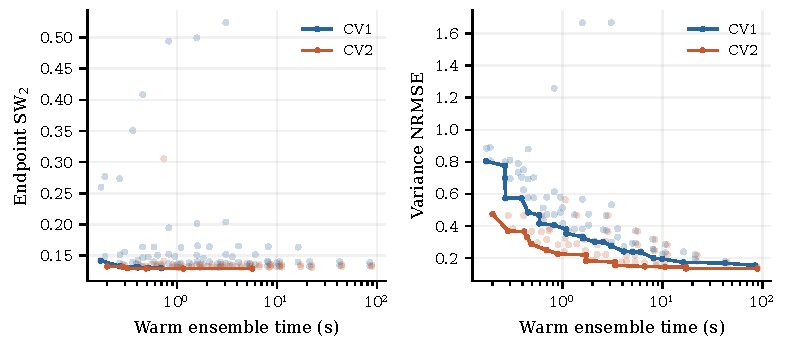
\includegraphics[width=\linewidth]{figures/log1p_frontiers.pdf}
\par\smallskip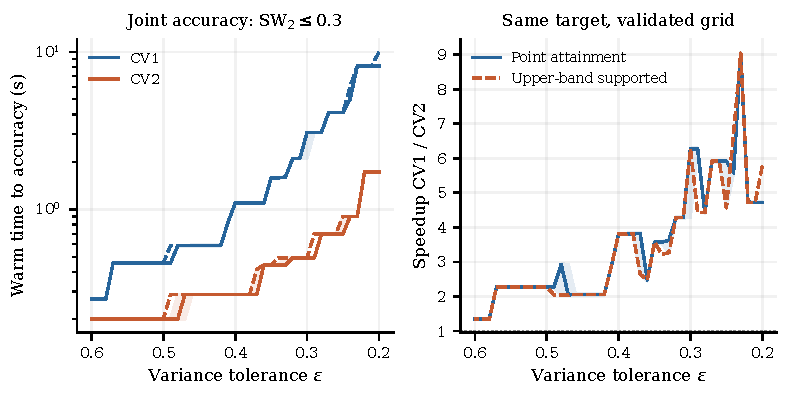
\includegraphics[width=\linewidth]{figures/log1p_joint_tta.pdf}
\caption{Validated accuracy--cost results for log-transformed Bank (P3A). Top: marginal SW$_2$ and variance-NRMSE frontiers against setup-inclusive warm JAX CPU ensemble time; faint points are all eligible $(n,h,K)$ configurations and lines the non-dominated boundaries. Bottom: joint time-to-accuracy (left) and CV1/CV2 speedup (right) with SW$_2\leq0.3$, across $41$ variance tolerances. Solid curves use point attainment and dashed curves supported attainment; shading gives approximate pointwise 95\% paired-bootstrap intervals.}\label{fig:log1p_frontier}\label{fig:log1p_joint}
\end{figure}
\FloatBarrier

\subsection{Dataset-size scaling (P3B)}\label{sec:exp_scaling}
We generate nested Bayesian logistic datasets with $d=20$, Gaussian features having AR(1) covariance $\Sigma_{ij}=0.5^{|i-j|}$, fixed alternating-sign coefficients scaled to population logit standard deviation $2$, and prior $N(0,I)$. The sizes $N\in\{2000,8000,32000,128000\}$ are exact prefixes of one maximum-size realization, without per-size restandardization. Each size has its own mode, full-H metric and approved references. Whitened SW$_2$ and a common relative variance definition avoid using the same absolute transport tolerance for posteriors of shrinking scale.

\paragraph{Noise scaling.}
At fixed minibatch size $n=16$, we enumerate observation contributions to the exact conditional gradient-noise MSE at $32$ reference locations per size; additional controlled whitened shells test remainder tails. The raw log--log slopes are $2.016$ for SGLD, $1.024$ for CV1 and $-0.001$ for CV2 (Figure~\ref{fig:noise_scaling}). These descriptive four-point trends agree qualitatively with the predicted raw orders under concentration and regularity conditions; they do not prove an asymptotic equality. Preconditioned slopes are $1.006$, $0.013$ and $-1.018$, respectively. Since $P_N$ changes with $N$, raw and preconditioned scaling must not be conflated.

The largest feature norm grows from $8.06$ to $9.03$, while the maximum raw CV2 residual across reference locations falls to $0.021$ of its small-$N$ value. At a common whitened radius $\sqrt d$, the corresponding factor is $0.023$. In this Gaussian-design family, concentration dominates the observed extreme-feature growth. This finding does not extend automatically to heavy-tailed designs.
\begin{figure}[tb]
\centering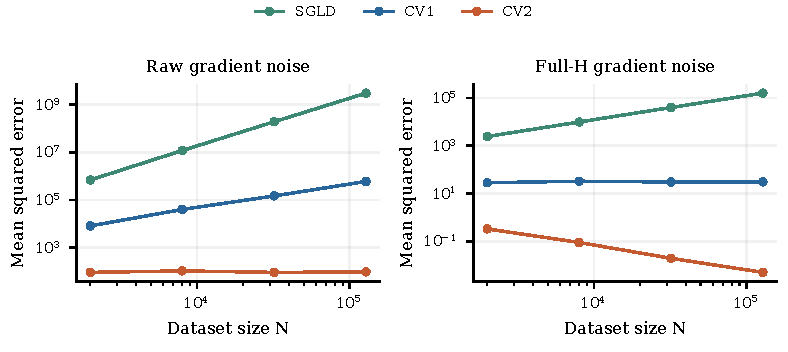
\includegraphics[width=\linewidth]{figures/noise_scaling.pdf}
\caption{Raw (left) and preconditioned (right) exact gradient-noise MSE against $N$ at fixed $n=16$, on one nested synthetic realization. All observations are enumerated at $32$ reference locations per size.}\label{fig:noise_scaling}
\end{figure}

\paragraph{Optimized time-to-accuracy.}
For each $N$, the same bounded pilot/selection rules choose independent validation candidates, without importing Bank-optimal parameters. There are $192$ pilot and $192$ validation runs per size, $1536$ in total. All validation runs are complete with no failures or censoring. We emphasize the cross-$N$ joint time-to-accuracy and speedup summary in the main text; the complete marginal frontier point clouds for each $N$ appear in Appendix~\ref{app:n_frontiers}. CV2 remains faster at the four representative accuracy targets (Table~\ref{tab:n_scaling}), but its speedup decreases between $N=2000$ and $128000$ by approximately $33\%,61\%,49\%,25\%$ for variance thresholds $0.5,0.4,0.3,0.2$. The trajectory across sizes need not be monotone, and CV2 is not faster at every one of the $41$ thresholds for every size. No eligible configuration at any size violates SW$_2\leq0.3$. At every size, CV2's selected configuration uses the smallest tested batch, $n=1$, at $40$ or $41$ of the $41$ warm thresholds, and also the earliest checkpoint, $K=128$, at $23$--$25$ of them; within this grid, further CV2 variance reduction cannot always be converted into saved work.
\begin{table}[tb]
\centering\small
\caption{Synthetic dataset-size scaling: setup-inclusive warm point-attainment speedup CV1/CV2, with whitened SW$_2\leq0.3$.}\label{tab:n_scaling}
\begin{tabular}{rrrrr}
\toprule
Variance & $N=2000$ & $8000$ & $32000$ & $128000$ \\
\midrule
0.50 & 2.146 & 2.137 & 1.825 & 1.441 \\
0.40 & 3.684 & 3.432 & 1.807 & 1.428 \\
0.30 & 4.326 & 4.762 & 2.845 & 2.210 \\
0.20 & 4.363 & 4.638 & 4.205 & 3.273 \\
\bottomrule
\end{tabular}
\par\smallskip{\footnotesize At variance threshold $0.3$, approximate 95\% intervals in increasing-$N$ order are $[3.438,4.391]$, $[4.260,5.362]$, $[2.830,2.860]$, $[2.141,2.259]$.}
\end{table}

\begin{figure}[tb]
\centering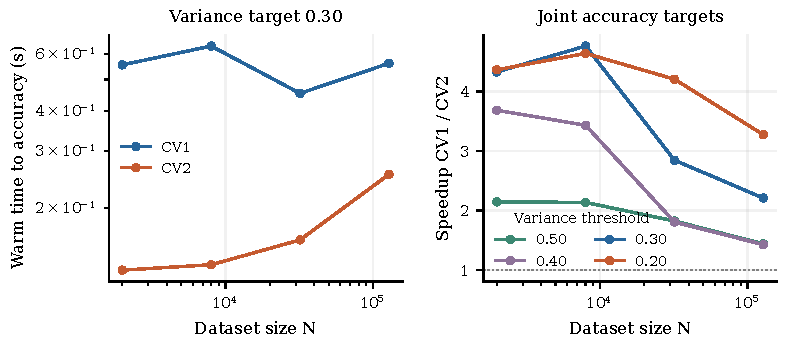
\includegraphics[width=\linewidth]{figures/n_efficiency.pdf}
\caption{Setup-inclusive warm point-attainment time-to-accuracy with independent tuning and validation at each $N$, requiring SW$_2\leq0.3$. Left: times at variance target $0.3$. Right: CV1/CV2 speedups at four variance targets.}\label{fig:n_efficiency}
\end{figure}

\paragraph{Why does total speedup decline?}
A saved-prefix cost decomposition, requiring no new sampling, writes $T_m=A_m+K_mc_m$, where $A_m$ is attributed setup and $c_m$ is batched sampling time per step. At variance threshold $0.5$, sampling-only speedup stays approximately $2.21$--$2.26$, while setup-inclusive speedup falls from $2.15$ to $1.44$. The noise advantage itself grows much faster than either time advantage: from $N=2000$ to $128000$, the CV1/CV2 ratio of reference-location gradient-noise MSE rises from about $89$ to $6270$ in raw terms and from about $86$ to $6190$ after preconditioning, roughly $70$-fold. Together with CV2's selections at the smallest tested batch and often the earliest checkpoint, this pattern is consistent with gradient noise no longer limiting CV2's accuracy, so that further variance reduction cannot be converted into additional saved work within the tested grid. CV2's setup share rises from $5.5\%$ to $65.0\%$: the common additive mode/metric preparation cost increasingly dilutes its already faster sampling. At stricter targets, CV1's changed batch, step and iteration choices also narrow the work gap. At matched configurations, CV2/CV1 per-step timing ratios range only from $0.982$ to $1.071$; there is no observed large growth of CV2-specific overhead sufficient to explain the total decline. This is an accounting decomposition and observational timing control, not randomized causal attribution (Appendix~\ref{app:cost}).

\FloatBarrier
\paragraph{Full-gradient ULA comparison.}\label{sec:exp_ula}
To assess whether CV2's measured benefits extend beyond comparisons with first-order control variates, we conducted a review-motivated, two-stage extension against full-gradient ULA at $N=2000$ and $N=128000$. Configurations were selected in an exploratory pilot and then evaluated without reselection on eight independent held-out seeds with $512$ mode-start replicas each. All $136$ validation runs completed without failed replicas or censoring. At $N=128000$, the simultaneous upper bounds for all three methods satisfy SW$_2\leq0.3$ and relative variance NRMSE$\leq0.3$. Under setup-inclusive warm accounting, CV2 reaches this joint target in $0.247$ seconds, compared with $0.560$ for CV1 and $16.3$ for ULA. The corresponding CV1/CV2 and ULA/CV2 time ratios are $2.26$ (approximate paired bootstrap 95\% interval $[2.19,2.34]$) and $65.9$ ($[62.7,69.8]$). From the same reported times, CV1 is itself about $29$ times faster than ULA, so most of the ULA/CV2 ratio reflects control-variate minibatching in general; the CV1/CV2 ratio isolates the additional contribution of the second-order correction. At $N=2000$, the point-estimate ULA/CV2 ratio is $4.21$, but CV2's simultaneous upper variance bound is $0.310$, above the $0.3$ tolerance; only $68.9\%$ of paired bootstrap draws jointly attain the target. This smaller-endpoint comparison is descriptive, rather than evidence of simultaneous-supported target attainment.

The pilot freezes a separate $(h,n,K)$ policy for each cost convention and tolerance; failure to attain a target refers to that preselected policy, not every tested configuration. Warm time includes attributed mode fitting and actual full-Hessian/cache preparation but excludes JIT compilation; cold time additionally attributes shape-specific compilation in the shared process. Thus the extension supports a substantial advantage over the selected ULA policy at the tested large-data endpoint, rather than a universal speedup or an independently reoptimized held-out frontier. \par\begin{samepage}
The advantage over full-gradient sampling is conditional: at $N=2000$ it is not supported at the simultaneous level, and on original Bank (Section~\ref{sec:exp_accuracy}) only ULA reached the frozen joint target in the selected-step comparison.
\par\end{samepage}

In summary, P3B provides the prospectively frozen efficiency evidence. CV2 reaches the four representative joint targets $1.43$--$4.76$ times faster than CV1 at every tested $N$, but the advantage narrows as $N$ grows, because shared setup takes a growing share of total time and CV2's additional noise reduction stops translating into saved work.

\FloatBarrier
\subsection{Mixing efficiency and computational cost}\label{sec:exp_ess}
Sections~\ref{sec:exp_accuracy}--\ref{sec:exp_scaling} measure accuracy at fixed budgets or time to a joint accuracy target. This subsection adds a descriptive chain-efficiency summary from existing post-burn-in records. For seed $s$, let $E_s$ be the smallest coordinate bulk ESS over $C$ unthinned chains, each with $T$ retained draws after $B$ burn-in transitions. We report $E_s$ per setup-inclusive second and per counted observation-gradient call, as medians of per-seed ratios. A configuration is eligible only if every seed passes maximum rank-$\widehat R<1.01$ and minimum coordinate bulk and tail ESS of at least $400$, with no numerical failure and a fixed metric.

Table~\ref{tab:german_ess} compares CV1, CV2 and ULA at common full-H step $h=0.4$ on four German selection-stage seeds. CV2 has a similar minimum bulk ESS to CV1 ($3304$ versus $3262$), but lower setup-inclusive ESS per second ($4173$ versus $4597$); ESS per observation-gradient call is comparable. ULA's ESS per observation-gradient call is about $30$ times lower, because each of its steps uses all $1000$ observations, while its ESS per second remains within about $25\%$ of CV1's on this small dataset. Observation-gradient counts exclude Hessian work, which enters measured time; Hessian contributions and data-row visits are separate operation units, and we do not convert them into gradient equivalents.

These NumPy CPU diagnostics assess chain mixing, not posterior approximation accuracy, and do not form an optimized time-to-accuracy comparison; passing the mixing gate does not remove discretization bias. The principal P1--P3 endpoint and running-functional archives do not record within-chain autocorrelation, so comparable ESS is not available for the optimized studies. Appendix~\ref{app:ess_cost} lists all eight eligible configuration groups, including historical YearMSD settings with unequal chain budgets, and all $39$ excluded groups, among them identity SGLD and the adaptive controls.

\begin{table}[!htbp]
\centering\small
\caption{German Credit post-burn-in mixing diagnostics at fixed full-H $h=0.4$. Each displayed configuration passes all four selection-stage seeds; entries are medians across those seeds.}\label{tab:german_ess}
\setlength{\tabcolsep}{4pt}
\begin{tabular}{lrrr}
\toprule
Method & Min bulk ESS & ESS/s & ESS/obs. grad. \\
\midrule
CV1 & 3262.1 & 4596.9 & 0.004943 \\
CV2 & 3303.6 & 4172.5 & 0.005005 \\
ULA & 3304.9 & 3515.7 & 0.000165 \\
\bottomrule
\end{tabular}
\par\smallskip{\footnotesize Each seed uses four chains, $1000$ discarded burn-in transitions and $4000$ retained draws per chain. CV1/CV2 use batch $32$; ULA uses all $1000$ observations. The numerator is the smallest coordinate bulk ESS within each seed. Ratios are formed per seed before taking medians. Seconds include setup and burn-in; gradient counts exclude Hessian work, which is included in measured time.}
\end{table}

\FloatBarrier
\subsection{Gaussian verification (P4)}\label{sec:exp_gaussian}
A focused quadratic finite-sum check uses $N=256,d=10$, condition numbers $10$ and $10^4$, identity/full-H metrics, four paired seeds and $512$ replicas. CV2 explicitly evaluates the minibatch Taylor remainder. Across $32$ fixed-budget method runs, its maximum scaled gradient discrepancy from the full gradient is $3.54\times10^{-13}$ and its maximum whitened path discrepancy from ULA, under shared initialization and Gaussian innovations, is $4.62\times10^{-13}$. All numerical gates pass, with no failures.

Exact finite-step Gaussian laws isolate geometry and discretization. At $K=1024$ and $\kappa=10^4$, population $W_2$ is $2.604$ under identity versus $0.0822$ under full-H. At $\kappa=10$, the corresponding values are $0.0194$ and $0.0822$: full-H removes slow geometry but need not minimize final error under the common stability-coefficient rule. It retains discretization bias, and mode-start transient discrepancy can be nonmonotone. Empirical full optimal-transport distances and independent exact-vs-exact baselines are reported separately from these analytic population distances. No speedup conclusion is drawn from this verification (Appendix~\ref{app:gaussian}).

A historical YearPredictionMSD Gaussian-ridge study supplies a complementary real-data example: near-exact CV2 gradients do not overcome severely ill-conditioned identity geometry, whereas full-H arms pass the declared mixing checks. Appendix~\ref{app:year_geometry} preserves its chain-based evaluation, direct Gaussian control and limitations separately from the independent-replica efficiency studies.

\subsection{Experimental discussion}\label{sec:exp_discussion}
The experiments address three successive questions. First, does CV2 reduce stochastic-gradient noise as intended? In the nested synthetic family it does: raw and preconditioned noise-scaling slopes agree qualitatively with the predicted orders (Section~\ref{sec:exp_scaling}). Second, does that reduction save computation at matched accuracy? Under prospectively frozen tuning and validation, CV2 reaches the four representative joint targets $1.43$--$4.76$ times faster than CV1 at every tested $N$, and at $N=128000$ it is also substantially faster than the selected full-gradient ULA policy. On the transformed Bank target, validated speedups are $2.27$--$6.27$. Third, when does the benefit fail to appear?

Three conditions emerge. First, stochastic-gradient noise must materially limit the chosen posterior accuracy: variance reduction has little measurable time value when discretization or a loose target dominates, as in the P2 synthetic targets, where every method meets the original loose target at the earliest checkpoint, and in P3B, where a roughly $70$-fold growth in the noise ratio leaves sampling-only speedup at variance threshold $0.5$ near $2.2$. Second, the observation-level remainder distribution must permit useful stable steps; global whitening does not remove every high-leverage contribution, as the original Bank failures show. Third, saved sampling work must outweigh preparation and competing-method retuning, which explains the declining setup-inclusive speedup in P3B. These conditions explain why the strongest computational evidence comes from independently validated optimized P3 comparisons, while P1/P2 and the original Bank results retain important null or unfavorable findings.

Posterior geometry is a prerequisite rather than a source of CV2's relative advantage in these experiments. All main comparisons share one fixed full-Hessian metric, and P4 and the YearMSD study show that exact gradients alone do not overcome ill-conditioned identity geometry. Overall, under a fixed geometry-correcting preconditioner, second-order control variates can translate improved stochastic-gradient precision into substantial time-to-accuracy savings, but only when gradient noise limits accuracy; rare high-leverage Taylor remainders and shared setup costs can erase or dilute the benefit. The experiments therefore support a conditional accuracy--cost benefit, rather than uniform superiority over first-order control variates.

\subsection{Scope and limitations}\label{sec:exp_limitations}
The following conditions apply throughout this section. References are approximate Metropolis-corrected HMC draws; passing the reference diagnostic gates is necessary for the reported rankings but does not prove an exact reference distribution. SW$_2$ is a finite-cloud projected discrepancy rather than certified population $W_2$, and finite-cloud reference-versus-reference discrepancies are reported but not subtracted as a bias correction. Bootstrap intervals use eight algorithm-seed clusters and condition on fixed references; simultaneous accuracy bands are approximately calibrated within their declared family and carry no joint guarantee across dataset sizes.

All optima are restricted to frozen, finite candidate grids. Minima selected among validation candidates remain potentially optimistic. The $41$ variance thresholds are strongly dependent rather than separate tests, and configuration changes between adjacent thresholds can make speedup curves nonmonotone. Absolute times depend on hardware and implementation: NumPy CPU, A100/T4 GPU and JAX CPU sessions, including the new ULA measurements, are not pooled into one ranking. Production minibatches in P1--P3 are drawn without replacement and use the fixed metric~\eqref{eq:exp_update} (Appendix~\ref{app:metrics}). Passing a chain mixing gate does not imply posterior accuracy. The P3A evidence concerns a transformed posterior whose transformation and tuning were both chosen after the original results, and the dataset-size study uses one nested Gaussian-design realization.

\section{Discussion}\label{sec:discussion}
The experiments distinguish a more accurate stochastic gradient from a more efficient sampler. Under fixed full-Hessian geometry, second-order correction can improve posterior variance estimates and the validated accuracy--cost frontier, but rare observation-level remainders can limit stable step sizes. Conversely, even favorable gradient-noise scaling need not produce increasing time savings: shared preprocessing and the competing method's tuning change the total cost. These conclusions concern the declared targets, finite search grids, accuracy metrics and implementations.

The transformed Bank result is a positive practical example, not a replacement for the negative original-target result. Transformation changes the posterior, and its effect cannot be separated from the subsequent tuning by comparing final speedups alone. Further generalization would require additional data-generating realizations and feature distributions. These observations distinguish gradient-oracle variance reduction from improvements in measured posterior accuracy and wall-clock cost.
\appendix
\section{Experimental protocols and reproducibility}\label{app:protocols}
This appendix gives protocol details for the experiment families in Table~\ref{tab:exp_overview}; their protocol classifications are not changed by the choice of displayed figures. Appendices~\ref{app:year_geometry}--\ref{app:reproduce} contain the historical YearPredictionMSD geometry study, the complete ESS tables and the reproduction assets.

\subsection{Targets, preprocessing and geometry}
German uses the frozen $61$-coordinate encoding without an intercept, prior precision $1$, and a fixed posterior metric. Bank uses reference-level categorical coding, standardized continuous features and an intercept. The $\log(1+\texttt{previous})$ sensitivity replaces and restandardizes only that continuous column; the winsorized version caps it at $22$, the declared $99.9\%$ quantile, affecting $45$ rows. Labels and other design columns are unchanged. The maximum standardized value decreases from approximately $119.1$ to $10.1$ and $12.0$ respectively. Each altered design has its own Gaussian-prior posterior: retaining the same prior form does not make this a posterior-preserving reparameterization.

Fixed-size synthetic logistic targets share $N=30{,}000,d=20$. Three have design covariance condition number $10^4$: correlated signal1, scaled signal1 and correlated signal3. The benign target has design condition number $10$. Measured posterior Hessian condition numbers are approximately $3097,3465,1660,9.65$. These targets differ in more than one posterior characteristic; their comparison does not identify a causal effect of condition number alone. P3B uses the distinct AR(1) mechanism described in the main text, no intercept and prior $N(0,I)$. Its data-generation and label-uniform seeds are $206000$ and $206001$; the coefficient vector and construction are recorded in the frozen configuration.

Constant-metric drift and noise both use the same $P$. Metric regularization is recorded separately from the exact prior contribution and from likelihood Taylor caches. The full-H likelihood cache can be reused when the metric already requires the Hessian; the saved runtime ledger, not an assumed theoretical operation equivalence, determines the reported setup. Identity/diagonal pilot arms are not substitutes for a complete independently validated preconditioning ablation on every logistic target.

\subsection{References and quality gates}\label{app:references}
References are approximate full-data, Metropolis-corrected HMC draws \citep{neal2012hmc}. Separate pools are used to check sensitivity and agreement; correlated HMC draws are not treated as iid bootstrap units. Rank-normalized convergence and bulk/tail ESS are assessed as in \citet{vehtari2021rank}. The principal gates require maximum $\widehat R<1.01$, minimum bulk and tail ESS at least $400$, no recorded divergences, minimum acceptance above $0.5$, and study-specific independent-pool agreement checks.

Original Bank initially fails: maximum $\widehat R$ is $1.0136/1.0144$ and minimum tail ESS $315/389$. An explicit reference-only amendment increases each pool from four chains with $256$ warmup and $1024$ retained draws per chain to $1024$ warmup and $8192$ retained draws. The original target, HMC scheme and quality gates remain unchanged; fresh reference seeds are $182010/182011$. Both longer pools pass, with maximum $\widehat R$ approximately $1.0004$, minimum bulk ESS above $28{,}000$, tail ESS above $13{,}000$, and no divergences. No Bank pilot is ranked before this gate passes.

For P3B, each $N$ has two pools of four chains, $1024$ warmup plus $8192$ retained draws per chain, eight leapfrog steps and warmup-only adaptation. Independent-pool agreement requires maximum mean-MCSE standardized difference below $4$ and relative covariance difference below $0.2$. All sizes pass the original gates. Transformed Bank constructs fresh approved references as well. German's original protocol additionally checks normalized functional MCSE and inter-reference functional disagreement; those original thresholds and reference-only baselines are retained in its configuration. A reference diagnostic pass is necessary for these rankings, not proof of stationarity or exact posterior truth.

\subsection{Metrics and estimator objects}\label{app:metrics}
Let $z=(\theta-\hat\theta)$ expressed in the declared posterior-standardized coordinates, and let $v_j$ be the reference variance of coordinate $j$. For seed $s$ and replica $r$, the ergodic coordinate-variance estimate through the declared checkpoint is $\widehat v_{srj}$. The later relative error is
\begin{equation}\label{eq:exp_relative_variance}
 E_s=\frac1d\sum_{j=1}^d\left\{\frac1R\sum_{r=1}^R
 \left(\frac{\widehat v_{srj}-v_j}{v_j}\right)^2\right\}^{1/2}.
\end{equation}
The P2/P3 variance estimates accumulate steps $1$ through $K$ without discarding a separate burn-in interval. Their error therefore measures finite-horizon, mode-start estimation rather than a post-burn-in stationary variance estimate; the chain ESS summary in Section~\ref{sec:exp_ess} uses a different retained-sample object. The reported error averages seeds; when both reference means must pass, the less favorable reference mean is used for eligibility. The original German criterion instead normalizes variance-functional errors by a frozen reference-calibration standard deviation. Its target $0.1$ and later relative targets $0.5$ or $0.1$ are therefore not equivalent. The cross-phase sensitivity recomputes the relative metric from saved functionals, without changing the original primary decision.

For SW$_2$, finite endpoint and reference clouds are projected onto fixed unit directions and one-dimensional empirical squared transport distances are averaged before taking a square root. Logistic production comparisons use the declared reference samples and projection resolution, with consistent $128$ directions in the later P3B pipeline. This is not full multivariate population $W_2$. Finite-cloud reference-vs-reference discrepancy is retained and not subtracted as if it were a known bias correction. P4 separately computes full equal-weight empirical optimal transport and an analytic Gaussian population distance.

At a common location, raw gradient-noise MSE is $\mathbb E\|\widehat g-g\|^2$. Preconditioned MSE is $\mathbb E\|P^{1/2}(\widehat g-g)\|^2$. In the row-vector implementation, $P=LL^\top$ and the squared norm is computed after right multiplication by $L$. Exact enumeration of centered observation residuals includes the without-replacement finite-population factor
\begin{equation}\label{eq:exp_finite_population}
 \frac{N^2(N-n)}{n(N-1)}\frac1N\sum_{i=1}^N
 \|r_i-\bar r\|^2,
\end{equation}
or the same norm transformed by $L$. Deterministic prior and anchor corrections cancel in conditional noise. Production P1--P3 minibatches are without replacement; this differs from the iid minibatch notation in Section~\ref{sec:method}. P4 deliberately uses iid with-replacement batches as a standalone quadratic check.

\subsection{Search, validation and uncertainty}\label{app:selection}
Original P2 synthetic selection uses $144$ runs, four new seeds and $R=128$. It freezes $h=0.1$ for all three methods in the first, second and fourth regimes; in correlated signal3, CV1 uses $h=0.05$ and CV2/ULA $0.1$. Held-out uses $96$ runs ($4$ targets, $3$ methods, $8$ seeds), $R=512$, minibatch $32$, and checkpoints $128,512,2048,8192$. Thus the strong-signal comparison is of selected configurations, not a same-step isolation. The four primary variance contrasts at $K=2048$ use $19{,}999$ paired-seed bootstrap draws and $98.75\%$ individual Bonferroni-adjusted intervals. Other P2 metrics and checkpoints use exploratory intervals. Original Bank freezes CV1 $h=0.05$, CV2 $0.00625$, and ULA $0.1$ after its own bounded pilot, not synthetic-optimal settings. P1's primary SW$_2$ target, $0.1133721697$, is the frozen reference-only baseline median plus $0.01$.

Optimized log-transformed Bank uses six batch sizes and initial steps $h=c/L_P$, with $c$ in\[\{0.0015625,0.00625,0.025,0.1,0.4,1.6\}.\] One declared refinement round permits at most two extra steps per method/batch. Pilot seeds choose stable non-dominated candidates using warm/cold time and both accuracy measures, at most two per batch and twelve per method. The $24$ candidates are frozen before validation seeds $205200$--$205207$. Validation horizon $4096$ is set by the declared pilot rule rather than extended after viewing validation. Each P3B size follows the corresponding frozen bounded pipeline, with fresh per-size configurations and seed audits; no transfer of a Bank optimum is assumed.

At variance threshold $\varepsilon$, point-attainment time minimizes declared mean cost among eligible configurations/checkpoints satisfying both reference accuracy means and SW$_2\leq0.3$. Supported time instead requires simultaneous upper accuracy bounds to pass. A minimum is conditional on the validated candidate grid; selecting it from validation data can remain optimistic. If only one method reaches the target, report that fact without an infinite or finite speedup. All $41$ thresholds from $0.20$ to $0.60$, in $0.01$ increments, are retained. Adjacent thresholds are strongly dependent, and checkpoint or configuration changes between them can produce nonmonotone speedup ratios.

P3 optimized inference uses $10{,}000$ paired whole-seed bootstrap resamples, preserving all configuration/checkpoint dependence within the resampled seed. Minima are reselected within each bootstrap draw. Not-Reached mass and conditional intervals are retained. Approximate simultaneous accuracy bands cover the declared eligible configuration/checkpoint, two-reference, two-metric family. The log-transformed Bank critical max-statistic is $3.336$. Calibration with eight seed clusters is approximate and conditional on fixed references; per-$N$ bands do not establish a joint across-$N$ coverage guarantee. Point and supported choices can differ: at log-transformed Bank variance threshold $0.2$, warm speedup is $4.723$ for point-attainment and $5.776$ for supported choices. Figure~\ref{fig:thresholds_app} retains the full curve.
\begin{figure}[tb]
\centering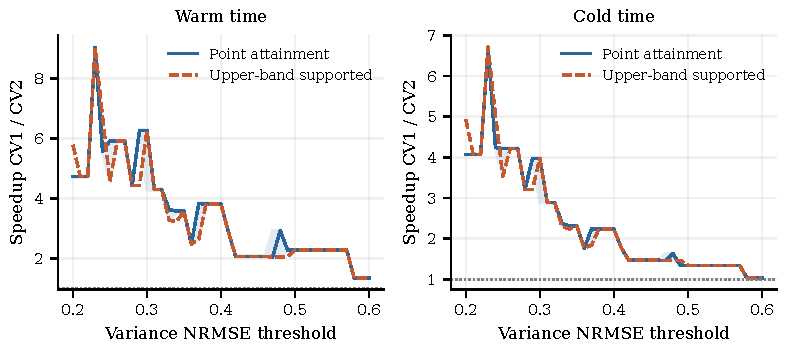
\includegraphics[width=\linewidth]{figures/log1p_thresholds.pdf}
\caption{Complete log-transformed Bank threshold analysis: CV1/CV2 speedup at all $41$ variance-NRMSE thresholds for warm (left) and cold (right) time, under point and supported attainment.}\label{fig:thresholds_app}
\end{figure}

\subsection{Failures and diagnostic side experiments}\label{app:failures}
Nonfinite states or excessive declared standardized radius trigger a numerical failure; a typical frozen radius limit is $100\sqrt d$. Failed replicas are never removed to score a surviving subset. Eligibility follows each original protocol: early P1/P2 comparisons retain valid pre-failure prefixes, whereas optimized P3A/P3B exclude a complete configuration at every checkpoint if any validation seed fails or is incomplete at the full horizon. Retrospectively applying one rule to all phases would change the experiments.

German's twelve diagnostic replays reproduce original streams and $64$ replicas through $2048$. At full-H coefficient $0.8$, CV2 has $14/64$ failures in each seed, beginning at iterations $82$ and $467$; coefficient $0.4$ and paired CV1/ULA controls show no failures in this replay. Independent gradient, Hessian and noise calculations agree to roundoff. The large stochastic-gradient-error drift dominates the tested terminal proposals; this is evidence of a stability limitation at those steps, not an identified implementation bug.

For practical Li2016-style controls \citep{li2016psgld}, zero-initialized raw-gradient RMSprop uses $\alpha=0.99$ and $\epsilon=10^{-5}$ in the detailed German replay, with prior/CV correction excluded from metric accumulation and the adaptive correction term omitted. At coefficient $0.256$, Li-pCV2 has $27/64$ and $33/64$ failures, starting at iteration $3$; paired Li-pCV1 does not fail. Sparse coordinates absent from early minibatches retain $D=1/\epsilon$, while CV2's full-data correction acts in those coordinates. These failures concern this exploratory zero-initialized, correction-omitted implementation and may reflect its design choices rather than a limitation of Li et al.'s method. Adaptive preconditioning is outside the primary comparison because the shared fixed metric controls posterior geometry, not because these runs establish method-level inferiority.


A subsequent bounded initialization sensitivity uses two fresh JAX seeds, $64$ replicas and $2048$ steps on the same German target. It holds $h=1.32\times10^{-5}$, $\alpha=.99$, $\epsilon=10^{-5}$ and batch $32$ fixed, pairing minibatch and Gaussian streams while changing only the initial accumulator. Li-pCV2 records $30/64$ and $29/64$ failures with zero initialization, versus $0/64$ in both runs with an independent $32$-minibatch anchor initializer. The Li-SGLD and Li-pCV1 controls record no failure under either initialization. These are new diagnostic streams, not exact replays of the earlier NumPy failures. They support initialization sensitivity of early stability, without establishing posterior accuracy, mixing or optimized adaptive efficiency; no further adaptive search is used for the primary comparison.

The Bank diagnostic first audits $61$ common states (anchor, reference, trajectory, stress and selected failure states). The high-leverage sensitivity reconstructs all $28$ failed-replica trigger batches, preserving the dependence induced by common seeds. The one other triggering observation is also retained; observation $29182$ is not asserted to cause every failure. Counterfactual replacement does not remove observations from the inference target. The feature-sensitivity stage then changes the target explicitly and uses fresh references and validation seeds.

Intermediate log-transformed Bank tests fix $n=16,h=0.025$ and vary $K\in\{128,256,384,512\}$. Both methods first meet the loose target at $K=256$, giving warm speedup $0.876$ with interval $[0.830,0.913]$, favoring CV1. A post-result threshold sweep finds different rankings at tighter criteria. These fixed-configuration results are preserved rather than replaced by the later optimized positive example. They explain why a common threshold or one favorable configuration is insufficient to determine an optimized frontier.

\subsection{Runtime and scaling decomposition}\label{app:cost}
The Gaussian prior is evaluated exactly once per stochastic-gradient call; its curvature is included once in the full posterior metric. Shared anchor preparation is measured once and attributed to each independently compared ensemble using it. CV1 also pays for full-H metric construction. Component records may aggregate Hessian assembly, inversion and noise factorization; where they do, no unmeasured separate timings are invented. Warm/cold differences reflect actual compilation/cache attribution. In P2, identical synthetic signatures reuse the compilation cache after the first target; later cold timings are not fresh-process costs.

For selected prefixes, let $Q_m=K_mc_m$ denote measured sampling time and $A_m$ the attributed mode/prepare time. The identity
\begin{equation}\label{eq:exp_cost_identity}
 \frac{T_1}{T_2}=\frac{K_1}{K_2}\frac{c_1}{c_2}
 \frac{1+A_1/Q_1}{1+A_2/Q_2}
\end{equation}
is bookkeeping, not a fitted model. The P3B supplement checks $87$ unique selected prefixes, $696$ seed-prefix records, $656$ decomposition identities and $164$ endpoint identities. Timing is per batched $512$-replica update, not serial single-chain cost.

At variance threshold $0.4$, CV1 changes batch $32\to16$ between endpoint dataset sizes. At $0.3$, it changes $(n,h,K)=(16,0.05,512)$ to $(16,0.1,384)$, while CV2 remains at $n=1,K=256$. At $0.2$, CV1 trades batch $16\to32$ for steps $2048\to1024$; CV2 remains at $n=1,K=1024$. These changes, plus shared setup dilution, explain why raw gradient-noise rates do not determine speedup alone. At the loose target, the best CV2 choices already sit on the tested minimum batch and earliest checkpoint; further variance reduction cannot necessarily save work within that grid. Figure~\ref{fig:cost_app} shows recorded components; because selected batches differ across accuracy targets and $N$, component differences are not pure per-step algorithmic overhead. Removing setup is a sensitivity analysis, not a replacement official ranking. Correction-only microbenchmark timings were not saved.
\begin{figure}[tb]
\centering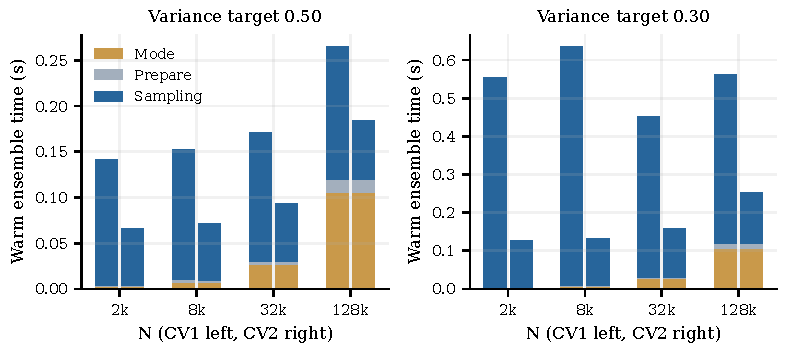
\includegraphics[width=\linewidth]{figures/cost_components.pdf}
\caption{Mode, preparation and sampling components of setup-inclusive warm time for the selected P3B configurations at variance targets $0.5$ (left) and $0.3$ (right); within each $N$, CV1 is left and CV2 right.}\label{fig:cost_app}
\end{figure}

\FloatBarrier
\subsection{Per-size validated accuracy--cost frontiers}\label{app:n_frontiers}
Figure~\ref{fig:n_frontiers_app} retains all $168$ eligible configuration/checkpoint points per synthetic dataset size, with separate SW$_2$--time and variance--time boundaries. The same non-dominance and full-horizon eligibility rules apply as for transformed Bank. Times include setup; errors use the worse reference mean, with common axis limits across sizes. Marginal boundaries can select different configurations and do not establish joint attainment. The main-text speedups impose both requirements through~\eqref{eq:exp_joint_time}. All optima are grid-restricted and subject to validation-selection optimism. Cold costs and supported choices remain in the full analysis.
\begin{figure}[p]
\centering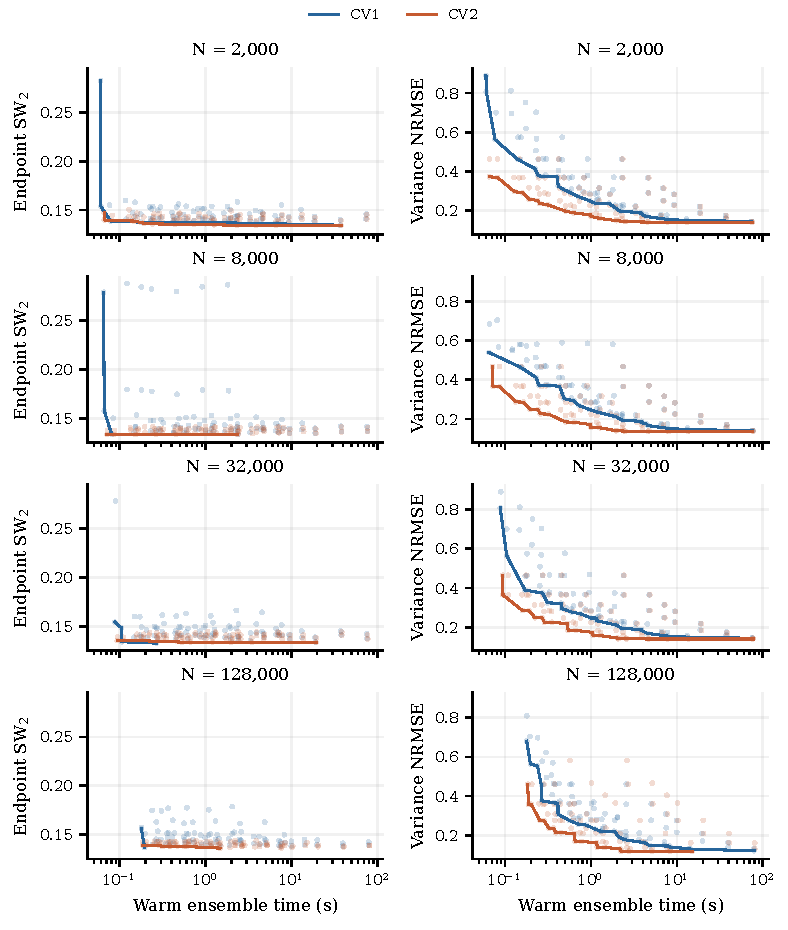
\includegraphics[width=\linewidth,height=0.78\textheight,keepaspectratio]{figures/p3b_full_frontiers.pdf}
\caption{Marginal accuracy--cost comparisons for P3B at $N=2000,8000,32000,128000$ (rows): endpoint whitened SW$_2$ (left) and relative variance NRMSE (right) against setup-inclusive warm time. Faint points are all eligible configuration/checkpoints and lines the non-dominated boundaries; axes are common across sizes.}\label{fig:n_frontiers_app}
\end{figure}
\FloatBarrier
\subsection{Gaussian verification details}\label{app:gaussian}
The tridiagonal-covariance Gaussian target is realized as a finite quadratic sum with heterogeneous rank-one observation Hessians. The actual precision $Q=X^\top X+\lambda_0 I$ and linear term $b=X^\top y$ define the exact posterior $N(Q^{-1}b,Q^{-1})$. The exact mode is supplied through a recorded dense solve, not a hidden optimizer. CV2 is compared against an independent cached quadratic full-gradient oracle, while its own kernel explicitly evaluates the sampled remainder. Batch size is $16$, iid with replacement; checkpoints are $0,16,64,256,1024$, and sampler seeds are $207100$--$207103$.

With $P=I$ or $Q^{-1}$ and $hL_P=0.1$, the finite-step covariance follows the exact Gaussian transition law. Gradient and whitened path discrepancy gates are $10^{-10}$ and $10^{-8}$; a deliberately conservative empirical covariance-to-finite-law check uses Frobenius error divided by $\sqrt d$ at most $0.5$. Observed maximum is $0.1731$. Raw CV2 gradient MSE is $1.469\times10^{-29}$ at $\kappa=10$ and $1.378\times10^{-24}$ at $10^4$, numerical roundoff rather than material stochastic variance. Figure~\ref{fig:gaussian_app} shows analytic transport and covariance error, including stationary discretization bias.
\begin{figure}[tb]
\centering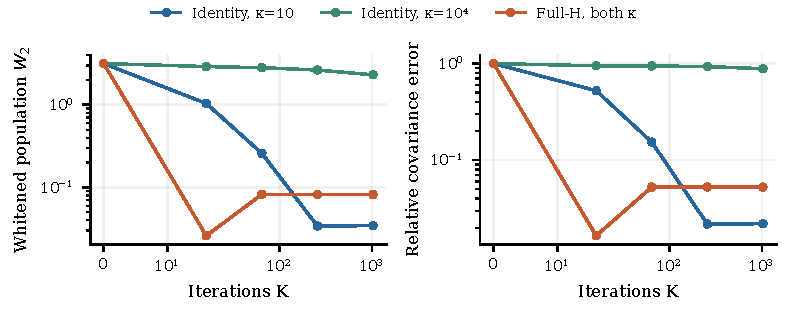
\includegraphics[width=\linewidth]{figures/gaussian_law.pdf}
\caption{Exact Gaussian transport and covariance under the common stability-coefficient rule. Full-H curves coincide across condition numbers; finite-step discretization bias remains.}\label{fig:gaussian_app}
\end{figure}

Empirical full $W_2$ uses exact equal-weight assignment between $512$ endpoints and $512$ independent exact draws, with an independent exact-vs-exact comparison retained as a finite-cloud baseline. It is neither a Gaussian fit nor a sliced approximation. Analytic and empirical distances are reported separately, in original and whitened coordinates. Verification timings include measured setup and shared pre-generated random-input construction; transfer of inputs into JAX is synchronized before timing but not separately attributed. ULA's cached quadratic oracle and CV2's explicit remainder are deliberately different verification workloads, not a production speed comparison.

% Integrated Appendix A.9--A.11; former standalone supplementary material.
\subsection{Historical YearPredictionMSD geometry study}\label{app:year_geometry}
This completed historical study is retained as a real-data geometry diagnostic, not as an additional main efficiency benchmark. We use the official $463{,}715$ training rows and $90$ features of YearPredictionMSD \citep{bertin2011year}, without feature standardization or an intercept, a $N(0,I)$ coefficient prior and fixed Gaussian observation variance $100$. The resulting posterior is Gaussian with analytically available sufficient statistics. Its precision condition number is $5.23\times10^6$. For these quadratic observation losses, CV2 coincides with the full gradient up to floating-point error: calibration checks give maximum relative discrepancy $1.10\times10^{-10}$. This does not test a nonquadratic Taylor approximation.

\paragraph{Frozen settings and evaluation object.}
Eight fresh paired seeds ($1000$--$1007$) each run four overdispersed chains, initialized at the declared posterior scale $2$, with $1000$ warmup transitions per chain. The historical implementation uses $\theta'=\theta-(s/2)P\widehat g+\sqrt{s}\,L\zeta$, so its saved step parameter $s$ corresponds to $h=s/2$ in~\eqref{eq:exp_update}. Identity CV1/CV2 use $s=2.2486761328\times10^{-12}$, batch $32$ and $4000$ retained draws per chain. Full-H CV1 uses $s=0.1$, batch $128$ and $20{,}000$ retained draws; full-H CV2 uses $s=0.3$ or $0.6$, batch $128$ and $4000$ retained draws. Parameters and budgets are frozen before these seeds. The full-H metric is the exact posterior covariance; it is held fixed.

Historical SW$_2$ uses $512$ spaced retained draws ($128$ per chain) against $1024$ independent exact Gaussian draws, with frozen calibration whitening and $512$ fixed directions. This evaluates a time-correlated chain-sample distribution, not the mode-start iterate law. Table values are seed medians; moments use all retained draws. For the frozen transform $W_{\mathrm{cal}}$, the errors are
\[
 E_\mu=\frac{\|(\bar\theta-\mu)^\top W_{\mathrm{cal}}\|}{\sqrt d},\qquad
 E_\Sigma=\frac{\|W_{\mathrm{cal}}^\top(\widehat\Sigma-\Sigma)W_{\mathrm{cal}}\|_F}{d}.
\]
Covariance uses the retained sample count as denominator. The normalization $E_\Sigma$ differs from P4's Frobenius error divided by $\sqrt d$ (Appendix~\ref{app:gaussian}).
\begin{table}[tb]
\centering\small
\caption{Historical YearPredictionMSD geometry study. Accuracy and time columns are seed medians; diagnostic columns give the worst $\widehat R$ and smallest bulk ESS over eight seeds. Passing requires $\widehat R<1.01$ and bulk ESS$\geq400$. SW$_2$ uses 512 spaced chain draws versus 1024 independent exact draws in frozen calibration-whitened coordinates; covariance normalization is defined in the text. Budgets and legacy step parameters differ across arms.}\label{tab:year_geometry}
\begin{tabular}{lrrrrrr}
\toprule
Arm & SW$_2$ & Cov. error & Time (s) & Max $\widehat R$ & Min ESS & Pass \\
\midrule
Identity, CV1 & 1.1039 & 1.1688 & 0.85 & 4.3087 & 4 & 0/8 \\
Identity, CV2 & 1.1048 & 1.1672 & 1.18 & 4.3079 & 4 & 0/8 \\
Full-H, CV1 ($s=.1$) & 0.1214 & 0.0248 & 6.91 & 1.0060 & 1636 & 8/8 \\
Full-H, CV2 ($s=.3$) & 0.1075 & 0.0229 & 2.05 & 1.0096 & 925 & 8/8 \\
Full-H, CV2 ($s=.6$) & 0.1353 & 0.0246 & 2.09 & 1.0043 & 2199 & 8/8 \\
Direct Gaussian & 0.0958 & 0.0079 & 0.13 & --- & iid & --- \\
\bottomrule
\end{tabular}
\end{table}


\paragraph{Geometry, mixing and discretization.}
Both identity arms fail the historical mixing criterion in all eight seeds despite CV2's near-exact gradient. They are budget-censored controls, not validated posterior approximations. At the frozen identity step, the exact linear-Gaussian transition gives a slowest-mean-direction e-fold time of approximately $5.23\times10^7$ transitions; this is an analytic time scale, not an observed finite-run convergence time. All full-H arms pass the table's criterion. Thus this real-data quadratic example complements the controlled Gaussian ablation: eliminating stochastic-gradient noise does not remove a geometry bottleneck.

Passing a mixing gate is not sufficient for accuracy. Increasing full-H CV2 from $s=0.3$ to $0.6$ improves its bulk ESS but increases median SW$_2$ from $0.1075$ to $0.1353$. Its seed-paired mean SW$_2$ difference is $+0.0263$ (approximate 95\% bootstrap interval $[0.0253,0.0276]$); the exact ULA stationary variance inflation is $8.1\%$ at $s=0.3$ versus $17.6\%$ at $s=0.6$. CV1's longer full-H run has slightly lower standardized mean error than CV2 at $s=0.3$ ($0.0234$ versus $0.0302$). The historical full-H CV2--CV1 SW$_2$ contrast is $-0.0131$ ($[-0.0165,-0.0100]$), but it compares different fixed steps and chain budgets, not an optimized matched-accuracy frontier. These conditional intervals use $20{,}000$ bootstrap resamples of only eight seed pairs, with fixed reference/scoring construction.

\paragraph{Direct sampling and cost limitations.}
The direct Gaussian control includes sufficient-statistic setup and $16{,}000$ independent draws ($512$ scored). Its median SW$_2$ is $0.0958$ and time approximately $0.13$ seconds. This finite-cloud comparison is not a zero-error floor or a bias correction to subtract. Direct sampling is substantially cheaper for this conjugate target; an MCMC preference is not implied.

Historical CPU times include the sufficient-statistic anchor, CV caches, metric inverse/factorization and four-chain transitions, excluding loading/scoring. CV1 retains $80{,}000$ draws versus CV2's $16{,}000$: the time difference is not a same-budget or optimized time-to-accuracy comparison. These timings remain outside the A100/JAX CPU/P3 rankings. Original records are preserved; no new sampling or tuning is added.

\clearpage
\subsection{Post-burn-in ESS and computational cost}\label{app:ess_cost}
\paragraph{Evaluation object and normalization.}
This appendix uses existing chain records, separately from the endpoint and ergodic-functional accuracy studies. For seed $s$, let $E_s$ be the smallest coordinate bulk ESS in the original collection of $C$ unthinned chains, each with $T$ retained draws after discarding $B$ burn-in transitions. We compute $E_s/(CT)$, $E_s/[C(T+B)]$, $E_s/t_s$ and $E_s/G_s$, where $t_s$ and $G_s$ are the setup-inclusive seconds and counted observation-gradient calls for that same chain collection. Table summaries take medians of these per-seed quantities; they are not ratios of medians. Measured setup includes required anchor, cache and metric preparation, followed by burn-in and sampling. Reference construction, loading and scoring are excluded as declared in the original ledgers. Chain costs come from the diagnostic records, not from the adjacent replica-ensemble timing files.

Hessian contributions and data-row visits remain separate operation units: ESS per observation-gradient call is not a complete computational-cost measure. All displayed German full-H settings record $18000$ observation-Hessian contributions, including mode/metric work; historical Year CV2 records an additional $463715$ likelihood-Hessian contributions, while Year CV1 has zero separately counted such contributions in its sufficient-statistic ledger. Their measured preparation costs remain included in seconds. No conversion to artificial gradient-equivalent counts is made.

\paragraph{Eligible configurations and study boundaries.}
German uses selection-stage seeds $242200$--$242203$, four chains, $B=1000$ and $T=4000$. Each configuration is eligible for descriptive throughput only if every seed passes maximum rank-$\widehat R<1.01$, minimum coordinate bulk and tail ESS at least $400$, with no recorded numerical failure and a fixed metric. The five eligible German settings and three eligible historical Year settings are all retained in Table~\ref{tab:ess_eligible}; this is not a selection of the best ESS/s rows. Section~\ref{sec:exp_ess} shows the common-$h=0.4$ German comparison, with batch $32$ for CV1/CV2 and full-data ULA.

Year uses eight historical seeds and the unequal chain budgets in Section~\ref{app:year_geometry}. Its saved diagnostic and cost summaries permit normalization, but that runner did not save the raw retained chains. Those ESS values are therefore source-verified; German's and the earlier short-chain diagnostics were independently recomputed from saved unthinned chains. Year retains the historical step symbol $s=2h$. Neither study is merged with GPU or JAX frontier timings, and the table does not estimate a global optimized ranking or significant method differences.
\begin{table}[tb]
\centering\small
\caption{Complete set of configurations eligible for descriptive ESS throughput: all seeds pass the chain gates. Studies remain separate. $E$ is the within-seed minimum coordinate bulk ESS; metric columns are medians of per-seed values or ratios.}\label{tab:ess_eligible}
\setlength{\tabcolsep}{4pt}
\begin{tabular}{lrrrrrr}
\toprule
Setting & Pass & $E$ & $E/(CT)$ & $E/[C(T+B)]$ & $E$/s & $E$/grad. \\
\midrule
\multicolumn{7}{l}{\textit{German selection diagnostics: four seeds}} \\
CV1, $h=.4$ & 4/4 & 3262.1 & 0.2039 & 0.1631 & 4596.9 & 0.004943 \\
CV2, $h=.2$ & 4/4 & 1415.8 & 0.0885 & 0.0708 & 1782.4 & 0.002145 \\
CV2, $h=.4$ & 4/4 & 3303.6 & 0.2065 & 0.1652 & 4172.5 & 0.005005 \\
ULA, $h=.2$ & 4/4 & 1443.8 & 0.0902 & 0.0722 & 1542.4 & 0.000072 \\
ULA, $h=.4$ & 4/4 & 3304.9 & 0.2066 & 0.1652 & 3515.7 & 0.000165 \\
\multicolumn{7}{l}{\textit{Year historical geometry: eight seeds}} \\
CV1, $s=.1$ & 8/8 & 1677.4 & 0.0210 & 0.0200 & 240.5 & 0.000150 \\
CV2, $s=.3$ & 8/8 & 1017.4 & 0.0636 & 0.0509 & 479.9 & 0.000336 \\
CV2, $s=.6$ & 8/8 & 2374.2 & 0.1484 & 0.1187 & 1122.3 & 0.000785 \\
\bottomrule
\end{tabular}
\par\smallskip{\footnotesize $C=4$ throughout. German has $B=1000,T=4000$. Year has $B=1000$, $T=20000$ for CV1 and $4000$ for CV2, with historical $s=2h$. Full-H is fixed in all displayed settings. Year ESS is source-verified; German ESS was recomputed from saved unthinned chains. Different steps, budgets and historical timings preclude a common optimized ranking.}
\end{table}

\FloatBarrier

\paragraph{Incomplete mixing and coverage.}
Table~\ref{tab:ess_excluded} retains every one of the $39$ configuration groups excluded from reliable throughput comparison, including settings with only one passing seed, identity SGLD and the practical adaptive controls. An adaptive metric is an additional reason for interpreting conventional ESS cautiously; the flagged adaptive groups also fail the numerical mixing gates. Ratios for failed groups are not used for ranking, and no successful-seed subset is substituted. Earlier synthetic/German short-chain studies are labelled separately from the current P1 protocol.
\begingroup
\small\setlength{\tabcolsep}{4pt}
\setlength{\LTcapwidth}{\textwidth}
\makeatletter\def\fnum@table{\tablename~\thetable}\makeatother
\begin{longtable}{lrrrrl}
\caption{All configurations excluded from reliable ESS-throughput comparison. Pass counts retain every seed. Diagnostic columns give the worst rank-$\widehat R$ and smallest bulk/tail ESS across seeds and coordinates, rather than the medians in Table~\ref{tab:ess_eligible}. No efficiency ratios are assigned to these groups.}\label{tab:ess_excluded}\\
\toprule
Setting & Pass & Max $\widehat R$ & Min bulk & Min tail & Flag \\
\midrule
\endfirsthead
\multicolumn{6}{l}{\textit{Table \thetable\ continued}} \\
\toprule
Setting & Pass & Max $\widehat R$ & Min bulk & Min tail & Flag \\
\midrule
\endhead
\midrule\multicolumn{6}{r}{\textit{Continued on next page}}\\
\endfoot
\bottomrule
\endlastfoot
\multicolumn{6}{l}{\textit{German P1 selection diagnostics}} \\*
CV1, $h=0.05$ & 0/4 & 1.0267 & 236.6 & 495.5 & M \\
CV1, $h=0.1$ & 1/4 & 1.0131 & 595.5 & 1167.8 & M \\
CV2, $h=0.1$ & 1/4 & 1.0123 & 578.3 & 1041.0 & M \\
ULA, $h=0.1$ & 1/4 & 1.0123 & 585.7 & 1069.8 & M \\
Identity SGLD, $c=0.05$ & 0/4 & 4.2817 & 4.3 & 10.8 & M \\
Identity SGLD, $c=0.2$ & 0/4 & 2.8736 & 4.6 & 10.7 & M \\
Li-CV1, $\alpha=0.99,c=0.256$ & 0/4 & 3.3316 & 4.4 & 10.8 & M+A \\
Li-CV2, $\alpha=0.9,c=0.016$ & 0/4 & 4.3264 & 4.3 & 10.7 & M+A \\
Li-SGLD, $\alpha=0.99,c=0.256$ & 0/4 & 2.6065 & 4.7 & 10.8 & M+A \\
Li-SGLD, $\alpha=0.9,c=0.064$ & 0/4 & 3.7517 & 4.3 & 10.7 & M+A \\
\multicolumn{6}{l}{\textit{Historical Year geometry}} \\*
Identity CV1 & 0/8 & 4.3087 & 4.2 & 10.6 & M \\
Identity CV2 & 0/8 & 4.3079 & 4.2 & 10.6 & M \\
\multicolumn{6}{l}{\textit{Earlier German short-chain study}} \\*
CV1 & 0/2 & 3.8456 & 4.4 & 11.0 & M \\
CV2 & 0/2 & 3.8385 & 4.4 & 11.0 & M \\
pCV1 & 0/2 & 4.0177 & 4.4 & 11.0 & M+A \\
pCV1 (fixed diagonal) & 0/2 & 4.0048 & 4.4 & 11.2 & M \\
pCV2 & 0/2 & 4.0399 & 4.4 & 11.0 & M+A \\
pCV2 (fixed diagonal) & 0/2 & 4.0217 & 4.4 & 11.1 & M \\
pSGLD & 0/2 & 3.9895 & 4.4 & 11.0 & M+A \\
pSGLD (fixed diagonal) & 0/2 & 3.9717 & 4.4 & 10.7 & M \\
SGLD & 0/2 & 3.8377 & 4.4 & 11.0 & M \\
\multicolumn{6}{l}{\textit{Earlier high-dimensional synthetic short chains}} \\*
CV1 & 0/1 & 2.9948 & 5.6 & 13.7 & M \\
CV2 & 0/1 & 2.1885 & 6.3 & 14.5 & M \\
pCV1 & 0/1 & 2.3639 & 6.1 & 13.7 & M+A \\
pCV1 (fixed diagonal) & 0/1 & 2.2687 & 6.3 & 14.6 & M \\
pCV2 & 0/1 & 2.3484 & 6.1 & 13.7 & M+A \\
pCV2 (fixed diagonal) & 0/1 & 2.1623 & 6.4 & 14.5 & M \\
pSGLD & 0/1 & 3.5223 & 5.4 & 13.7 & M+A \\
pSGLD (fixed diagonal) & 0/1 & 2.9053 & 5.7 & 13.7 & M \\
SGLD & 0/1 & 2.9972 & 5.6 & 13.5 & M \\
\multicolumn{6}{l}{\textit{Earlier low-dimensional synthetic short chains}} \\*
CV1 & 0/2 & 1.6144 & 6.8 & 25.1 & M \\
CV2 & 0/2 & 1.6141 & 6.9 & 25.1 & M \\
pCV1 & 0/2 & 2.1672 & 5.3 & 23.6 & M+A \\
pCV1 (fixed diagonal) & 0/2 & 1.6414 & 6.8 & 23.4 & M \\
pCV2 & 0/2 & 2.1626 & 5.3 & 23.7 & M+A \\
pCV2 (fixed diagonal) & 0/2 & 1.6340 & 6.8 & 24.0 & M \\
pSGLD & 0/2 & 2.1957 & 5.2 & 15.5 & M+A \\
pSGLD (fixed diagonal) & 0/2 & 1.5748 & 7.1 & 19.7 & M \\
SGLD & 0/2 & 1.5534 & 7.2 & 20.3 & M \\
\end{longtable}
\endgroup
\noindent\footnotesize M: at least one seed fails a numerical mixing gate. A: the metric also adapts throughout sampling, so conventional stationary-chain ESS is exploratory. The adaptive rows describe the tested initialization, accumulator and correction-omission choices only; they do not establish inferiority or general instability of Li et al. (2016). Adaptive metrics are outside the primary geometry-controlled comparison. The fixed-diagonal historical arms are distinct from the principal fixed full-H framework. For German identity and Li rows, $c$ is the original planning coefficient; it is not substituted for the public step $h$. No failed or nonmixing seed is removed to make a setting eligible.\normalsize


The audit reconstructs $105$ saved chain collections and extracts $40$ historical Year diagnostic/cost collections. The principal P1--P3 endpoint and running-functional archives do not identify within-chain autocorrelation ESS. Accordingly, this supplements the original ESS-per-cost request without claiming a reliable baseline-complete nonquadratic comparison for every experiment. It cannot replace SW$_2$, variance NRMSE or the frozen time-to-accuracy evaluation.

\FloatBarrier
\subsection{Reproduction assets and audit trail}\label{app:reproduce}
The reproducibility package contains frozen configurations, generated tables, full-precision numerical source mappings and figure provenance. Original datasets, HMC pools, per-run endpoints/functionals, failure records and full threshold analyses are retained in the research archive. The evidence registry links the experiment families to their detailed reports and numerical files. The compact manuscript package retains the selected source records; it does not substitute for the complete raw archives.

Historical Gaussian/YearMSD checks remain supporting material rather than additional nonquadratic efficiency evidence. The experimental conclusions are limited by approximate fixed references, eight algorithm-seed clusters, finite candidate grids, one nested synthetic data realization and hardware-dependent timing.

\bibliographystyle{ba2}
\bibliography{references}
\end{document}
